\documentclass[palatino, classical, simple name]{einfart}

\nolinenumbers% Enable line numbers

%%================================
%% Import toolkit
%%================================
\usepackage{ProjLib}
\usepackage{longtable}  % breakable tables
\usepackage{booktabs}
\usepackage{hologo}     % more TeX logo
\usepackage{multicol}
\usepackage{relsize}
\usepackage{float}
\usepackage{blindtext}
\usepackage{unicode-math}
\usepackage{fontawesome5}
\usepackage{xcolor}
\UseLanguage{Chinese}

%%================================
%% For typesetting code
%%================================
\usepackage{listings}
\definecolor{maintheme}{RGB}{70,130,180}
\definecolor{forestgreen}{RGB}{21,122,81}
\definecolor{lightergray}{gray}{0.99}
\lstset{language=[LaTeX]TeX,
    keywordstyle=\color{maintheme},
    basicstyle=\ttfamily,
    commentstyle=\color{forestgreen}\ttfamily,
    stringstyle=\rmfamily,
    showstringspaces=false,
    breaklines=true,
    frame=lines,
    backgroundcolor=\color{lightergray},
    flexiblecolumns=true,
    escapeinside={(*}{*)},
    % numbers=left,
    numberstyle=\scriptsize, stepnumber=1, numbersep=5pt,
    % firstnumber=last,
}
\providecommand{\meta}[1]{$\langle${\normalfont\itshape#1}$\rangle$}
\lstset{moretexcs=%
    {linenumbers,nolinenumbers,part,parttext,chapter,section,subsection,subsubsection,frontmatter,mainmatter,backmatter,tableofcontents,href,
    color,NameTheorem,CreateTheorem,cref,DNF,UseLanguage,UseOtherLanguage,AddLanguageSetting,maketitle,address,curraddr,email,keywords,subjclass,thanks,dedicatory,TheDate,ProjLib,qedhere
    }
}
\lstnewenvironment{code}%
{\setstretch{1.07}\LocallyStopLineNumbers%
\setkeys{lst}{columns=fullflexible,keepspaces=true}%
}
{\ResumeLineNumbers}
\lstnewenvironment{code*}%
{\setstretch{1.07}\LocallyStopLineNumbers%
\setkeys{lst}{numbers=left,columns=fullflexible,keepspaces=true}%
}
{\ResumeLineNumbers}

%%================================
%% tip
%%================================
\usepackage[many]{tcolorbox}
\newenvironment{tip}[1][提示]{%
    \LocallyStopLineNumbers%
    \begin{tcolorbox}[breakable,
        enhanced,
        width = \textwidth,
        colback = paper, colbacktitle = paper,
        colframe = gray!50, boxrule=0.2mm,
        coltitle = black,
        fonttitle = \sffamily,
        attach boxed title to top left = {yshift=-\tcboxedtitleheight/2, xshift=.5cm},
        boxed title style = {boxrule=0pt, colframe=paper},
        before skip = 0.3cm,
        after skip = 0.3cm,
        top = 3mm,
        bottom = 3mm,
        title={\scshape\sffamily #1}]%
}{\end{tcolorbox}\ResumeLineNumbers}

%%================================
%% Names
%%================================
\providecommand{\minimalist}{\textsf{minimalist}}
\providecommand{\minimart}{\textsf{minimart}}
\providecommand{\minimbook}{\textsf{minimbook}}
\providecommand{\einfart}{\textsf{einfart}}
\providecommand{\simplivre}{\textsf{simplivre}}
\numberwithin{equation}{section}
%%================================
%% Titles
%%================================
\let\LevelOneTitle\section
\let\LevelTwoTitle\subsection
\let\LevelThreeTitle\subsubsection

%%================================
%% Newcommand
%%================================

\newcommand{\Z}[1]{\mathcal{Z}\left[#1\right]}
\newcommand{\ZF}[1]{{\mathcal{Z}}^{-1}\left[#1\right]}
\newcommand{\dv}[2]{\frac{{\rm{d}}{#1}}{{\rm{d}}{#2}}}
\newcommand{\dvn}[2]{\frac{{\rm{d}}^{#1}}{{\rm{d}}{#2}^{#1}}}
\newcommand{\highlight}[2]{\colorbox{#1!17}{#2}}
\newcommand{\varomega}{\symit{\omega}}
%%================================
%% Main text
%%================================
\begin{document}

\title{核反应堆控制复习要点}
\author{核工A002班 张恺}
\email{\href{2966895623@qq.com}{2966895623@qq.com}}
\date{\zhtoday,西安交通大学核科学与技术学院}

\maketitle

\begin{abstract}
    本资料以复习提纲的形式整理了《核反应堆控制》的复习要点,给出了每一章考试涉及的重点内容,并选出部分课后习题做了解答。着重强调的内容用灰色底色提醒,即\highlight{gray}{强调的内容};部分公式交叉引用,正文里表述“式(X.X)”中,点击编号即可跳转。本课程各类计算题的解答过程都比较繁琐,需要熟练掌握解题步骤,并细心解答。因本人水平有限,错漏之处在所难免,欢迎读者批评指正。您可以通过以下方式联系我:
    \begin{itemize}
        \item {\faGithub}:\,\href{https://github.com/Enriched-Uranium/Nuclear-Reactor-Control}{https://github.com/Enriched-Uranium/Nuclear-Reactor-Control}
        \item {\faWeixin}:\,XJTU-NEer
    \end{itemize}
\end{abstract}

\setcounter{tocdepth}{1}
{\setstretch{1.07}\tableofcontents}


\medskip

\section{物理基础}

\subsection{缓发中子}

在实际裂变过程中,约有$\beta$份额的裂变中子通过缓发中子先驱核衰变而来,并在瞬发中子产生后相当长一段时间才起作用,这部分中子称为缓发中子,它们对核反应堆的周期影响很大,使得核反应堆的控制成为可能。

考虑缓发中子,则中子平均寿命$\bar{l}$由瞬发中子寿命$l_0$与所有各组(通常分为6组)缓发中子寿命$(t_i + l_0)$的加权平均值,即

\begin{equation}
    \bar{l} = (1 - \beta) l_0 + \sum_{i=1}^{6} \beta_i (t_i + l_0)
\end{equation}

查${}^{235} {\rm U}$的数据,$l_0 \approx 10^{-4}\,{\rm s}$,$\displaystyle \sum_{i=1}^{6} \beta_i t_i \approx 0.1\,{\rm s}$,则$\bar{l} \approx 0.1\,{\rm s} \Rightarrow \Lambda = 0.1\,{\rm s}$。若反应性$\rho = 0.001$,则反应堆周期$T = \Lambda / \rho = 100\,{\rm s}$,即反应堆功率增加${\rm e}$倍的所需时间为$100\,{\rm s}$,完全可以使用移动控制棒的方法控制反应堆。

\subsection{反应性控制}

\begin{definition}[剩余反应性]
    堆芯中没有任何控制毒物时的反应性。
\end{definition}

\begin{definition}[后备反应性]
    冷态干净堆芯的剩余反应性。
\end{definition}

反应性控制的本质是维持堆内中子的平衡,即控制中子的产生、吸收和泄漏,具体控制手段如下。
\begin{enumerate}
    \item 中子吸收体移动控制:改变中子吸收率
    \begin{enumerate}
        \item 控制棒:控制速度快、灵活,反应性价值变化小,但对堆内中子注量率分布扰动大,对控制棒驱动机构的可靠性要求较高。
        \item 慢化剂中可溶性毒物:不对功率分布产生过大影响,但调节较慢,浓度不能过高(参照《核反应堆物理分析》第7章)。
        \item 可燃毒物棒:毒物含量岁燃耗加深而减小,第一循环结束时去掉。
    \end{enumerate}
    \item 慢化剂液位控制:改变中子产生率
    \item 燃料控制:改变中子产生率
    \item 反射层控制:改变中子泄漏率
\end{enumerate}

答题时,注意题目问的是“反应性控制的手段”(4种)还是“中子吸收体移动控制的手段”(3种)。

\subsection{核电厂稳态运行方案}

重点是冷却剂平均温度程序方案。
\begin{enumerate}
    \item 冷却剂平均温度随负荷成线性变化
    \begin{equation}
        T_{\rm av} = T_{\rm av0} + K P_{\rm H}
    \end{equation}
    \item 一回路或二回路的全部负担,由一回路和二回路共同承担
    \item 应通过向堆芯深处插入控制棒组件以补偿堆芯反应性的增加
\end{enumerate}

\subsection{习题选解}

本章所有习题均在上文给出了解答。

\section{线性离散系统的分析方法}

\subsection{连续信号的采样与重构}

\subsubsection{连续信号的采样}

\begin{equation*}
    f(t) \xrightarrow{\text{采样}} f^*(t)
\end{equation*}

原连续信号为$f(t)$,采样后的离散信号为$f^*(t)$,满足

\begin{equation}
    f^*(t) = \sum_{k=0}^{\infty} f(kt) \delta(t-kT) = f(t)p(t)
\end{equation}

即理想采样信号$f^*(t)$可以看成连续信号$f(t)$和理想采样脉冲序列$\delta_{\rm T}(t)$的乘积。

理想采样:忽略脉冲宽度$\tau$,即瞬时采样。

\begin{theorem}[采样定理]
    连续信号采样后产生的高频幅频谱与基本幅频谱不发生重叠的条件是
    \begin{equation}
        (\text{采样频率}) \omega_s \geqslant 2 \omega_c (\text{连续信号最高频率})
    \end{equation}
\end{theorem}

\subsubsection{采样信号的重构}

重构条件:
\begin{enumerate}
    \item 满足采样定理;
    \item 采用理想滤波器。
\end{enumerate}
重构的实质是把一串脉冲序列$f(0)$,$f(T)$,$\cdots$,$f(kT)$平滑成连续的信号$f(t)$,常用Taylor级数多项式外推。

\subsubsection{零阶保持器}

\begin{equation}
    f_k(t) = f(kT),\,kT \leqslant t < (k+1)T
\end{equation}

零阶保持器将$f^*(t)$在$kT$时的状态保持到$(k+1)T$到来之前,其传递函数为

\begin{equation}
    G_{H_0}(s) = \frac{1-{\rm{e}}^{-Ts}}{s}
\end{equation}

\subsection{$Z$变换与反$Z$变换}

$f(t)$的$Z$变换和$f^*(t)$的$Z$变换结果相同,即

\begin{equation}
    \Z{f(t)} = \Z{f^*(t)} = F(z) = \sum_{k=0}^{\infty} f(kT) z^{-k}
\end{equation}

反过来,\highlight{gray}{$F(z)$的反$Z$变换只能得到唯一的$f^*(t)$,但不能得到唯一的$f(t)$},即

\begin{equation}
    \ZF{F(z)} = f^*(t) = f(kT)
\end{equation}

此处涉及的计算需要多做习题,提高熟练度,也需要复习一下拉普拉斯变换的知识。

\subsubsection{$Z$变换的计算}

\begin{align}
    & F(z) = \sum_{i=1}^{n} \lim_{s\to s_i} (s - s_i)\frac{F(s) z}{z - {\rm{e}}^{Ts}} \\
    & F(z) = \sum_{i=1}^{n} \lim_{s\to s_i} \frac{1}{(m_i - 1)!} \dvn{m_i-1}{s} \left[(s-s_i)^{m_i} \frac{F(s) z}{z - {\rm{e}}^{Ts}}\right]
\end{align}

\subsubsection{$Z$反变换的计算}

\begin{align}
    & f(k) = \sum_{i=1}^{n} \lim_{z\to z_i} (z - z_i) F(z) z^{k-1} \quad k=1, 2, 3, \cdots \\
    & f(k) = \sum_{i=1}^{n} \lim_{z\to z_i} \frac{1}{(m_i - 1)!} \dvn{m_i-1}{z} \left[(z-z_i)^{m_i} F(z) z^{k-1}\right] \quad k=1, 2, 3, \cdots 
\end{align}

\subsubsection{$Z$变换求解差分方程}

对差分方程两边同时作$Z$变换,解出$Y(z)$后,求其$Z$反变换。

此处常用以下两个性质,并注意此时$T=1\,{\rm s}$

\begin{align}
    & \Z{f(t+nT)} = z^n F(z) - \sum_{j=0}^{n-1} z^{n-j} f(j) \\
    & \Z{\delta(k)} = 1
\end{align}

\subsection{线性离散系统的脉冲传递函数}

\begin{definition}[脉冲传递函数]
    在零初始条件下,一个环节或系统的输出序列$Z$变换与输入序列$Z$变换之比,用
    \begin{equation}
        G(z) = \frac{C(z)}{R(z)}
    \end{equation}
    来表示。
\end{definition}

线性离散系统的脉冲传递函数只与系统本身的结构参数与性能有关,\highlight{\gray}{与输入信号无关。}

\begin{enumerate}
    \item 系统含有保持器时
    \begin{equation}
        G(z) = \Z{G(s) G_H(s)}
    \end{equation}
    \item 串联环节
    \begin{figure}[H]
        \centering
        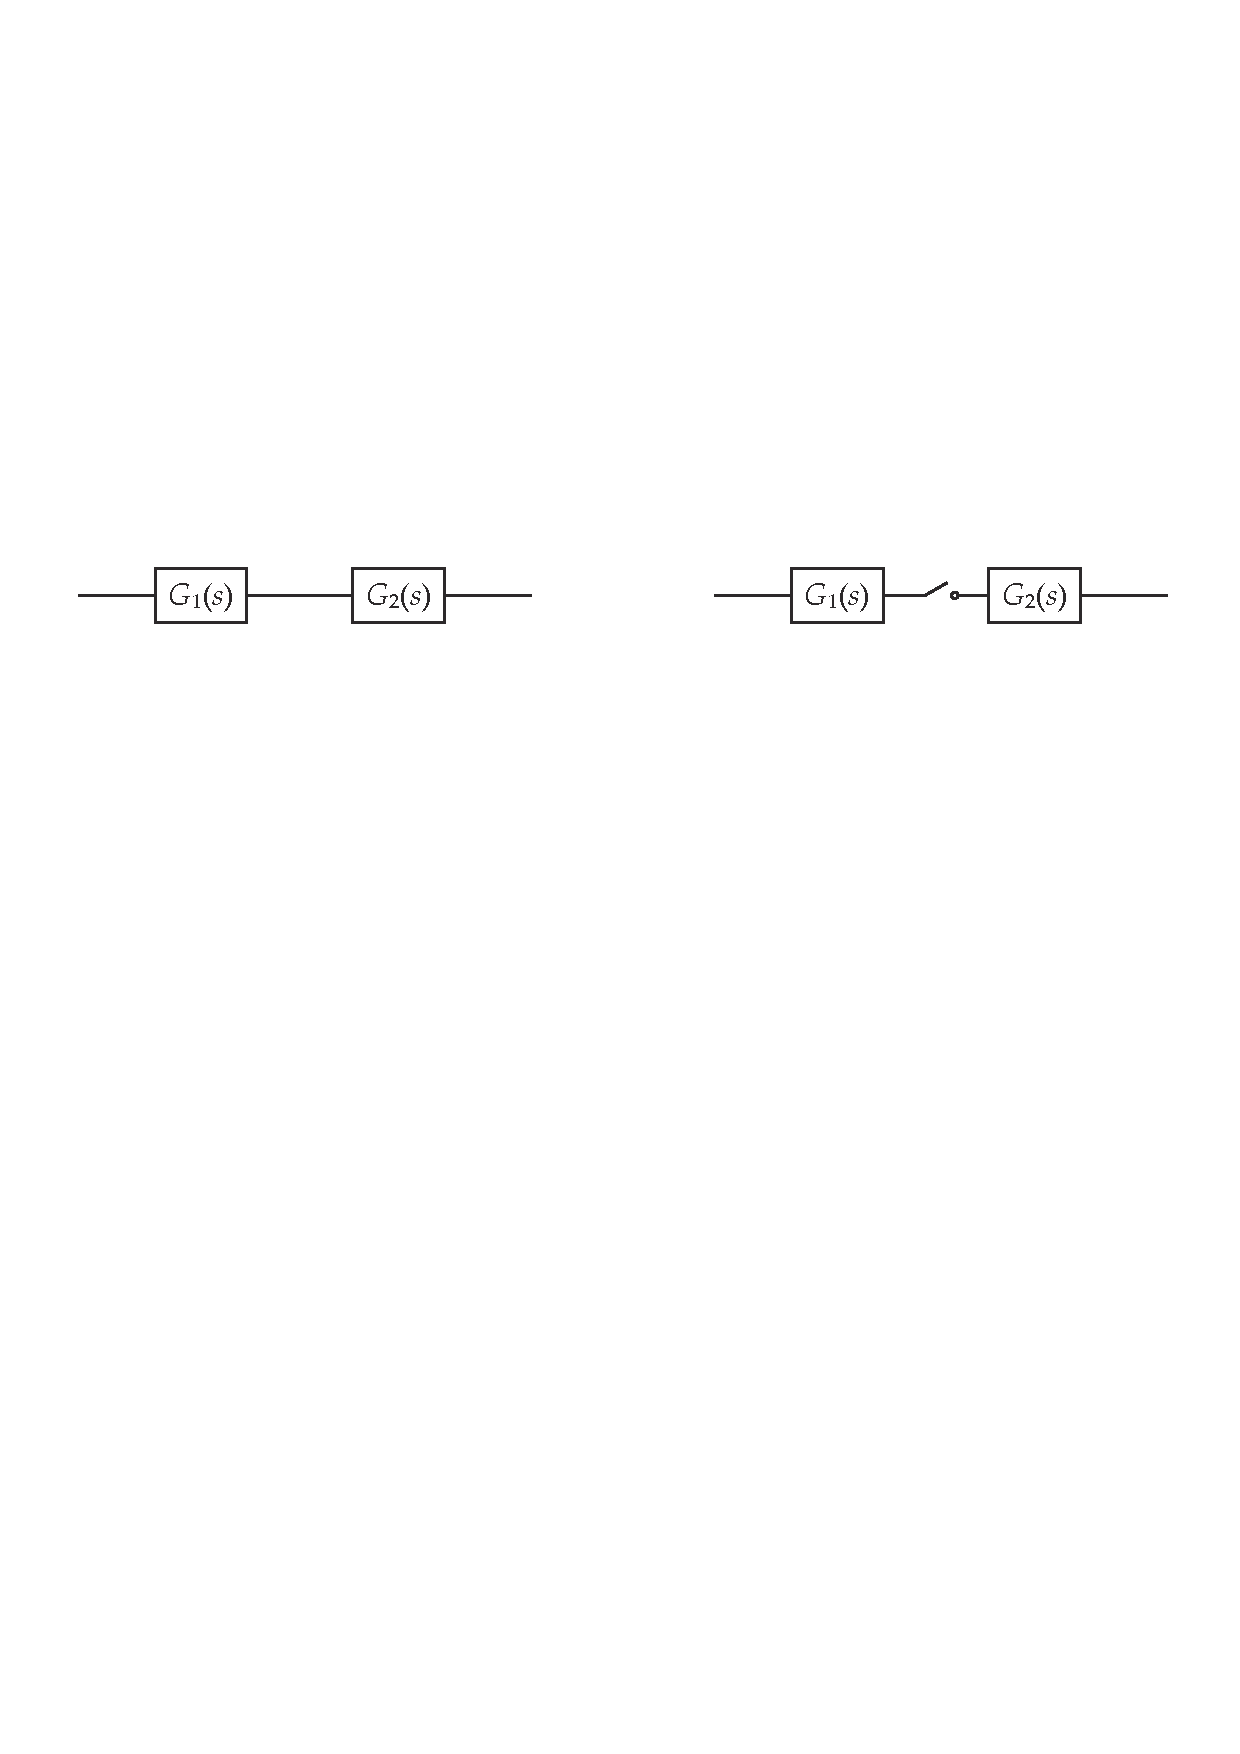
\includegraphics[scale=0.7]{figures/figure2.1.pdf}
    \end{figure}

    \begin{multicols}{2}
        \begin{equation}
            G(z) = \Z{G_1(s) G_2(s)}
        \end{equation}

        \begin{equation}
            G(z) = \Z{G_1(s)} \Z{G_2(s)}
        \end{equation}
    \end{multicols}
    \item 闭环脉冲传递函数
    此处注意对例2-12种$Z$变换过程的理解。
    \begin{figure}[H]
        \centering
        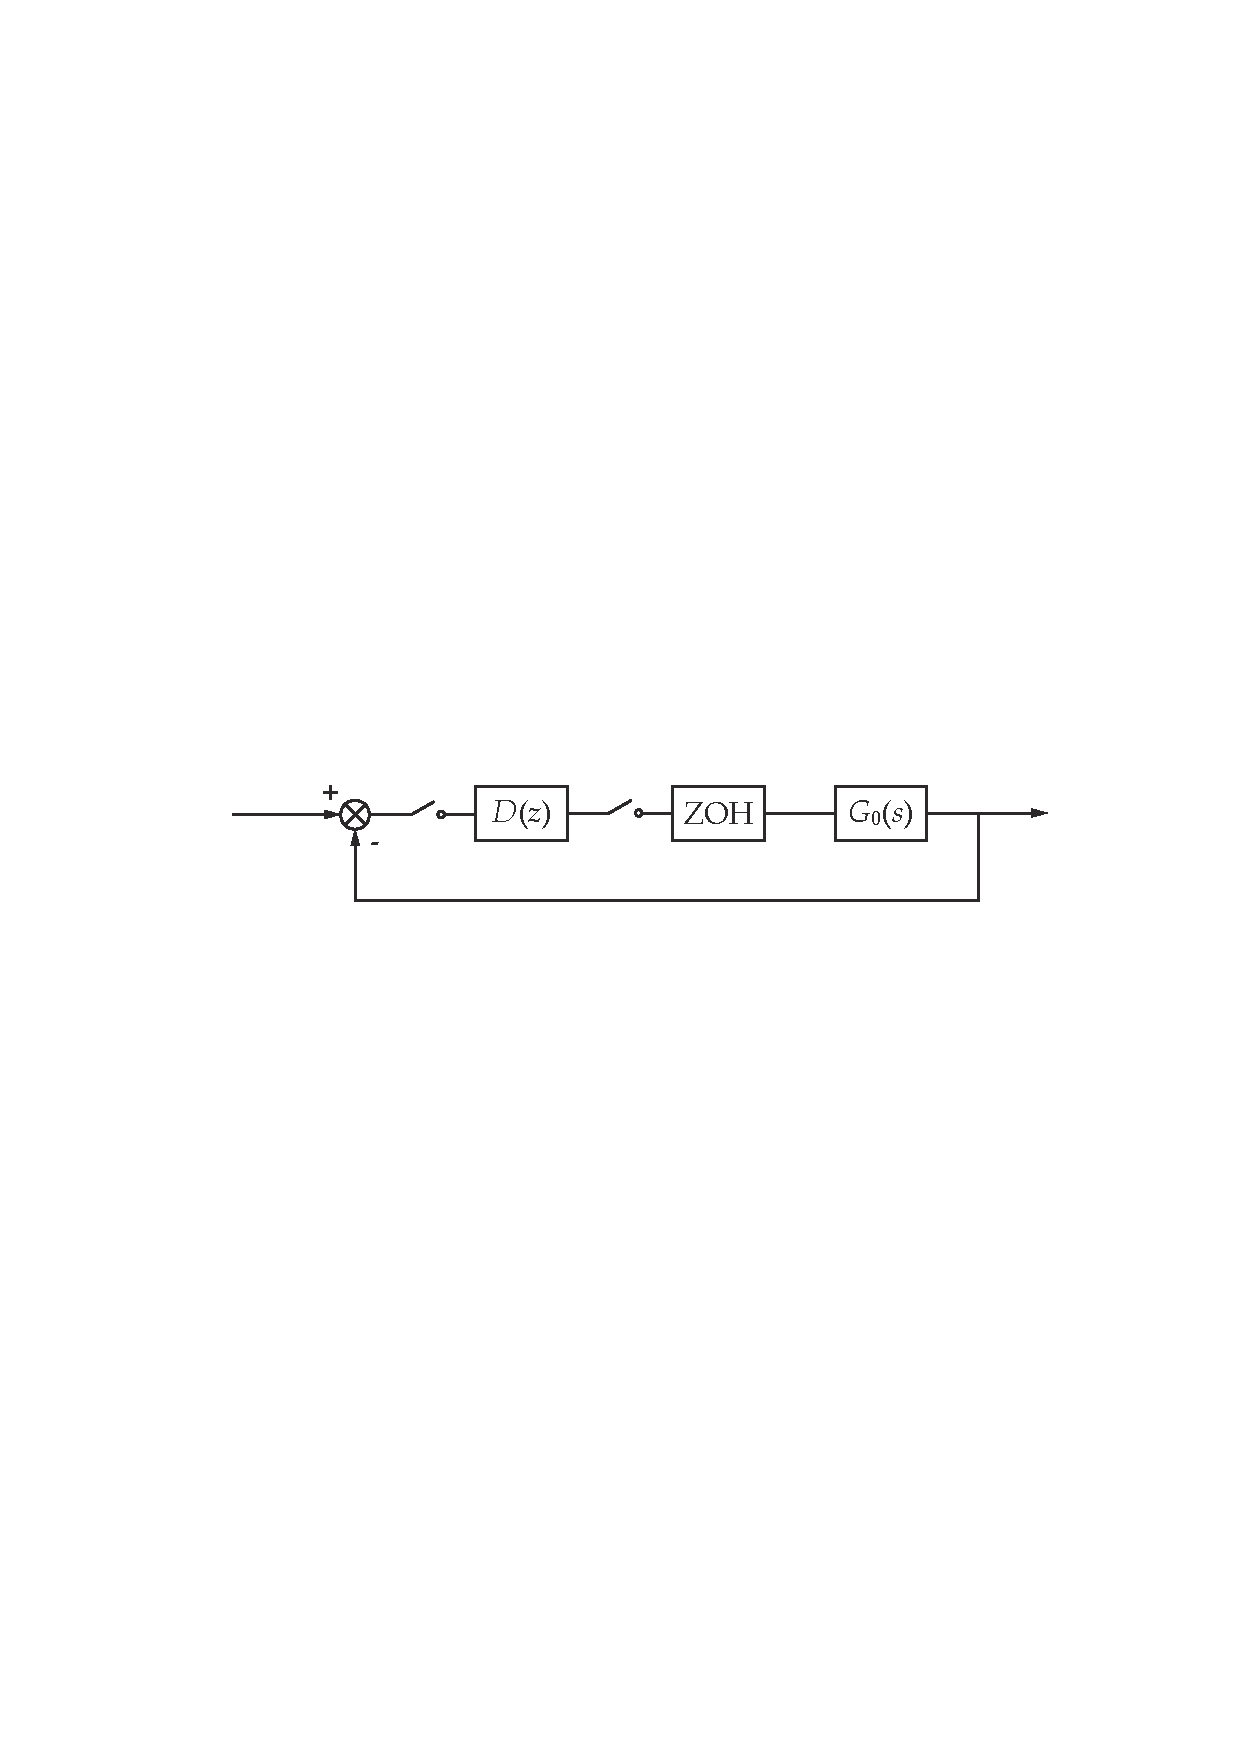
\includegraphics[scale=0.7]{figures/figure2.2.pdf}
    \end{figure}
    \begin{align}
        & G(z) = \Z{G(s)} = \Z{G_{H_0}(s) G_0(s)} \\
        & W(z) = \frac{C(z)}{R(z)} = \frac{D(z) G(z)}{1 + D(z)G(z)}
    \end{align}
\end{enumerate}

\subsection{习题选解}

\begin{exercise} % 2.3
    \begin{enumerate}
        \item \begin{align*}
            F(s)&= \mathcal{L}\left[f(t)\right] = \frac{1}{s+2a} \\
            F(z)&= \Z{F(z)} = \lim_{s \to -2a} (s+2a) \frac{z}{(s+2a)(z-{\rm e}^{Ts})} = \frac{z}{z-{\rm e}^{-2aT}}
        \end{align*}
        \item \begin{align*}
            F(s)&= \mathcal{L}\left[f(t)\right] = \frac{3}{s^2} \\
            F(z)&= \Z{F(s)} = \lim_{s \to 0} \frac{1}{(2-1)!} \dvn{}{s} \left[s^2 \cdot \frac{3z}{s^2 (z - {\rm e}^{Ts})}\right] = \lim_{s \to 0} \frac{3z T{\rm e}^{Ts}}{(z-{\rm e}^{Ts})^2} = \frac{3zT}{(z-1)^2}
        \end{align*}
        \item \begin{align*}
            F(s) = \mathcal{L}\left[f(t)\right] &= \frac{2}{(s+1)^2 + 4} \\
            F(z) = \Z{F(s)} &= \lim_{s \to -1-2j} (s+1+2j)\cdot \frac{2z}{[(s+1)^2+4] (z-{\rm e}^{Ts})} + \lim_{s \to -1+2j} (s+1-2j)\cdot \frac{2z}{[(s+1)^2+4] (z-{\rm e}^{Ts})} \\
                &= \lim_{s \to -1-2j} \frac{2}{s+1-2j} \cdot \frac{z}{z-{\rm e}^{Ts}} + \lim_{s \to -1+2j} \frac{2}{s+1+2j} \cdot \frac{z}{z-{\rm e}^{Ts}} \\
                &= \frac{1}{2j} \left[\frac{z}{z-{\rm e}^{(-1+2j)T}} - \frac{z}{z-{\rm e}^{-(1+2j)T}}\right]
        \end{align*}
        \item \begin{align*}
            F(z) = \Z{F(s)} &= \lim_{s \to -1} \frac{s+3}{s+2} \cdot \frac{z}{z-{\rm e}^{Ts}} + \lim_{s \to -2} \frac{s+3}{s+1} \cdot \frac{z}{z-{\rm e}^{Ts}} \\
            &= \frac{2z}{z-{\rm e}^{-T}} - \frac{z}{z-{\rm e}^{-2T}}
        \end{align*}
        \item \begin{align*}
            F(z) = \Z{F(s)} &= \lim_{s \to 0} \frac{1}{s^2+1} \cdot \frac{z}{z-{\rm e}^{Ts}} + \lim_{s \to -j} \frac{1}{s(s-j)} \cdot \frac{z}{z-{\rm e}^{Ts}} + \lim_{s \to j} \frac{1}{s(s+j)} \cdot \frac{z}{z-{\rm e}^{Ts}} \\
            &= \frac{z}{z-1} - \frac{z}{2(z-{\rm e}^{-jT})} - \frac{z}{2(z-{\rm e}^{jT})}
        \end{align*}
    \end{enumerate}
\end{exercise}

\begin{exercise} % 2.4
    \begin{enumerate}
        \item \begin{align*}
            F(s) = \ZF{F(z)} &= \lim_{z \to -1} \frac{z}{z-1} \cdot z^{k-1} + \lim_{z \to 1} \frac{z}{z+1} \cdot z^{k-1} \\
            &= \frac{1-(-1)^k}{2} \quad k = 1, 2, \cdots
        \end{align*}
        \item \begin{align*}
            F(s) = \ZF{F(z)} &= \lim_{z \to 1} \frac{1}{(2-1)!} \dvn{}{z} \left(\frac{z}{z-2} \cdot z^{k-1}\right) + \lim_{z \to 2} \frac{z}{(z-1)^2} \cdot z^{k-1} \\
            &= 2^k - k - 1 \quad k = 1, 2, \cdots
        \end{align*}
        \item \begin{equation*}
            F(s) = \ZF{F(z)} = \lim_{z \to 0} \frac{z^{k-1}}{z-0.2} + \lim_{z \to 0.2} \frac{z^{k-1}}{z} = 0.2^{k-2} \quad k = 1, 2, \cdots
        \end{equation*}
    \end{enumerate}
\end{exercise}

\begin{exercise} % 2.5
    此题差分方程应为
    \begin{enumerate}
        \item $y(k+2) - 5y(k+1) + 6y(k) = 0,\, y(0) = 0,\, y(1) = 1$
        \item $y(k+2) - 2y(k+1) + y(k) = k,\, y(0) = 0,\,y(1) = 0$
    \end{enumerate}

    \begin{enumerate}
        \item 两边同时$Z$变换,得
        \begin{equation*}
            z^2 Y(z) - z^2 y(0) - z y(1) - 5[z Y(z) - zy(0)] + 6Y(z) = 0
        \end{equation*}
        化简,得
        \begin{equation*}
            z^2 Y(z) - z - 5z Y(z) + 6Y(z) = 0
        \end{equation*}
        解得
        \begin{equation*}
            Y(z) = \frac{z}{(z-2)(z-3)}
        \end{equation*}
        做$Z$反变换,得
        \begin{align*}
            y(k) = \ZF{Y(z)} &= \lim_{z \to 2} \frac{z}{z-3} \cdot z^{k-1} + \lim_{z \to 3} \frac{z}{z-2} \cdot z^{k-1} \\
            &= 3^k - 2^k \quad k = 1, 2, \cdots
        \end{align*}
        \item 两边同时$Z$变换,得(此处$T=1\,{\rm s}$)
        \begin{equation*}
            z^2 Y(z) - z^2 y(0) - z y(1) - 2[z Y(z) - zy(0)] + Y(z) = \frac{z^{-1}}{(1-z^{-1})^2}
        \end{equation*}
        化简,得
        \begin{equation*}
            z^2 Y(z) - 2z Y(z) + Y(z) = \frac{z}{(z-1)^2}
        \end{equation*}
        解得
        \begin{equation*}
            Y(z) = \frac{z}{(z-1)^4}
        \end{equation*}
        做$Z$反变换,得
        \begin{align*}
            y(k) = \ZF{Y(z)} &= \lim_{z \to 1} \frac{1}{(4-1)!} \cdot \dvn{3}{z} \left(z\cdot z^{k-1}\right) \\
            &= \frac{k(k-1)(k-2)}{6} \quad k = 1, 2, \cdots
        \end{align*}
    \end{enumerate}
\end{exercise}


\section{线性控制系统的状态空间分析方法}

\subsection{状态空间表达式的建立}

\begin{align}
    & \dot{\symbfit{x}} = \symbfit{Ax} + \symbfit{B}u \\
    & y = \symbfit{Cx} + \symbfit{D}u
\end{align}

\subsubsection{由微分方程建立}

假如有

\begin{equation*}
    \dddot{y} + 6\ddot{y} + 11\dot{y} + 6y = 6u
\end{equation*}

则令

\begin{equation*}
    \begin{cases}
        x_1 = y \\ 
        x_2 = \dot{y} \\
        x_3 = \ddot{y}
    \end{cases} \Rightarrow \begin{cases}
        \dot{x}_1 = \dot{y} = x_2 \\
        \dot{x}_2 = \ddot{y} = x_3 \\
        \dot{x}_3 = -6x_1 - 11x_2 - 6x_3 + 6u
    \end{cases}
\end{equation*}

即

\begin{align*}
    \begin{bmatrix}
        \dot{x}_1 \\
        \dot{x}_2 \\
        \dot{x}_3
    \end{bmatrix} &= \begin{bmatrix}
        0 & 1 & 0 \\
        0 & 0 & 1 \\
        -6 & -11 & -6
    \end{bmatrix} \begin{bmatrix}
        x_1 \\
        x_2 \\
        x_3
    \end{bmatrix} + \begin{bmatrix}
        0 \\
        0 \\
        6
    \end{bmatrix} u \\
    y &= \begin{bmatrix}
        1 & 0 & 0
    \end{bmatrix} \begin{bmatrix}
        x_1 \\
        x_2 \\
        x_3
    \end{bmatrix}
\end{align*}

\subsubsection{由传递函数建立}

以
\begin{equation*}
    G(s) = \frac{Y(s)}{U(s)} = \frac{s^2 + 3s + 2}{s(s^2 + 7s + 12)}
\end{equation*}
为例。

\begin{enumerate}
    \item 直接转换法
    
    令
    \begin{equation*}
        \begin{cases}
            U(s) = (s^3 + 7s^2 + 12s) Q(s) \\
            Y(s) = (s^2 + 3s +2) Q(s)
        \end{cases}
    \end{equation*}

    两边同时作拉普拉斯反变换,得
    \begin{equation*}
        \begin{cases}
            u(t) = \dddot{q} + 7\ddot{q} + 12\dot{q} \\
            y(t) = \ddot{q} + 3\dot{q} + 2q
        \end{cases}
    \end{equation*}

    令
    \begin{equation*}
        \begin{cases}
            x_1 = q \\
            x_2 = \dot{q} \\
            x_3 = \ddot{q}
        \end{cases}
    \end{equation*}

    于是有
    \begin{equation*}
        \begin{cases}
            \dot{x}_1 = \dot{q} = x_2 \\
            \dot{x}_2 = \ddot{q} = x_3 \\
            \dot{x}_3 = \dddot{q} = -12x_2 - 7x_3 + u \\
            y = 2x_1 + 3x_2 + x_3
        \end{cases}
    \end{equation*}

    故
    \begin{align*}
        \begin{bmatrix}
            \dot{x}_1 \\
            \dot{x}_2 \\
            \dot{x}_3
        \end{bmatrix} &= \begin{bmatrix}
            0 & 1 & 0 \\
            0 & 0 & 1 \\
            0 & -12 & -7
        \end{bmatrix} \begin{bmatrix}
            x_1 \\
            x_2 \\
            x_3
        \end{bmatrix} + \begin{bmatrix}
            0 \\
            0 \\
            1
        \end{bmatrix} u \\
        y &= \begin{bmatrix}
            2 & 3 & 1
        \end{bmatrix} \begin{bmatrix}
            x_1 \\
            x_2 \\
            x_3
        \end{bmatrix}
    \end{align*}
    \item 部分分式法
    
    将原式分解为
    \begin{equation*}
        \frac{Y(s)}{U(s)} = \frac{1}{6}\frac{1}{s} - \frac{2}{3}\frac{1}{s+3} + \frac{3}{2}\frac{1}{s+4}
    \end{equation*}

    那么
    \begin{equation*}
        Y(s) = \frac{1}{6}\frac{1}{s}U(s) - \frac{2}{3}\frac{1}{s+3}U(s) + \frac{3}{2}\frac{1}{s+4}U(s)
    \end{equation*}

    令
    \begin{equation*}
        \begin{cases}
            X_1(s) = \frac{1}{s} U(s) \\
            X_2(s) = \frac{1}{s+3} U(s) \\
            X_3(s) = \frac{1}{s+4} U(s)
        \end{cases} \Rightarrow \begin{cases}
            sX_1(s) = U(s) \\
            sX_2(s) = -3X_2(s) + U(s) \\
            sX_3(s) = -4X_3(s) + U(s)
        \end{cases}
    \end{equation*}

    两边同时作拉普拉斯反变换,得
    \begin{equation*}
        \begin{cases}
            \dot{x}_1 = u \\
            \dot{x}_2 = -3x_2 + u \\
            \dot{x}_3 = -4x_3 + u \\
            y = \frac{1}{6}x_1 - \frac{2}{3}x_2 + \frac{3}{2}x_3
        \end{cases}
    \end{equation*}

    故
    \begin{align*}
        \begin{bmatrix}
            \dot{x}_1 \\
            \dot{x}_2 \\
            \dot{x}_3
        \end{bmatrix} &= \begin{bmatrix}
            0 & 0 & 0 \\
            0 & -3 & 0 \\
            0 & 0 & -4
        \end{bmatrix} \begin{bmatrix}
            x_1 \\
            x_2 \\
            x_3
        \end{bmatrix} + \begin{bmatrix}
            1 \\
            1 \\
            1
        \end{bmatrix} u \\
        y &= \begin{bmatrix}
            \frac{1}{6} & -\frac{2}{3} & \frac{3}{2}
        \end{bmatrix} \begin{bmatrix}
            x_1 \\
            x_2 \\
            x_3
        \end{bmatrix}
    \end{align*}

    \highlight{gray}{推荐使用部分分式法,}因为可以直接得到标准型。
    \item 传递函数与状态空间表达式之间的关系
    \begin{equation}
        G(s) = \frac{Y(s)}{U(s)} = \symbfit{C}(s\symbfit{I} - \symbfit{A})^{-1} \symbfit{B} + \symbfit{D} \label{G}
    \end{equation}
\end{enumerate}

\subsection{线性定常系统的线性变换}

经过此变换,将状态空间表达式转换为标准型,有利于判断线性定常系统的能控性和能观测性,标准型为
\begin{align}
    & \dot{\bar{\symbfit{x}}} = \bar{\symbfit{A}} \bar{\symbfit{x}} + \bar{\symbfit{B}}u \\
    & y = \bar{\symbfit{C}} \bar{\symbfit{x}} + \bar{\symbfit{D}}u
\end{align}

对于给定的非标准状态空间表达式,转换的一般步骤如下。但在此之前,最好复习一下线性代数的相关知识。

\begin{enumerate}
    \item 求特征值
    
    \begin{equation}
        \det(\lambda \symbfit{I} - \symbfit{A}) = 0 \Rightarrow \lambda_i
    \end{equation}

    并立即由此写出
    \begin{equation}
        \bar{\symbfit{A}} = \begin{bmatrix}
            \lambda_1 & & & \\
            & \lambda_2 & & \\
            & & \ddots &    \\
            & & & \lambda_n \\
        \end{bmatrix}
    \end{equation}
    \item 求特征向量
    
    \begin{equation}
        (\lambda_1 \symbfit{I} - \symbfit{A}) \symbfit{v}_i = 0 \Rightarrow \symbfit{v}_i
    \end{equation}

    线性变换矩阵由特征向量组成
    \begin{equation}
        \symbfit{P} = \begin{bmatrix}
            \symbfit{v}_1 & \symbfit{v}_2 & \cdots & \symbfit{v}_n
        \end{bmatrix}
    \end{equation}

    虽然可能大部分情况下,该矩阵均可逆,但最好计算一下$\det(\symbfit{P})$的值,说明“$\det(\symbfit{P}) \neq 0$,所以$\symbfit{P}$可逆”以求严谨,而且本来下一步也需要用到$\det(\symbfit{P})$的值。
    \item 求线性变换矩阵的逆矩阵
    
    \begin{equation}
        \symbfit{P}^{-1} = \frac{\symbfit{P}^*}{\det(\symbfit{P})}
    \end{equation}
    \item 求标准型系数矩阵
    
    \begin{align}
        & \bar{\symbfit{B}} = \symbfit{P}^{-1} \symbfit{B} \\
        & \bar{\symbfit{B}} = \symbfit{C} \symbfit{P} \\
        & \bar{\symbfit{D}} = \symbfit{D}
    \end{align}
\end{enumerate}

\subsection{线性定常系统的状态方程求解}

求解过程比较麻烦,结合例3-5掌握,需要细心。

\begin{align}
    & {\rm{e}}^{\symbfit{A}t} = \mathcal{L}^{-1} \left[(s \symbfit{I} - \symbfit{A})^{-1}\right] \\
    & x(t) = {\rm{e}}^{\symbfit{A}t} x(0) \\
    & x(t) = {\rm{e}}^{\symbfit{A}t} x(0) + \int_{0}^{t} {\rm{e}}^{\symbfit{A}(t-\tau)} \symbfit{B} \symbfit{u}(\tau) {\rm d} \tau
\end{align}

\subsection{能控性和能观测性}

对于给定的线性定常系统,有

\begin{enumerate}
    \item 状态完全能控 $\Longleftrightarrow$ $\bar{\symbfit{B}}$中无全零行
    \item 状态完全能观测 $\Longleftrightarrow$ $\bar{\symbfit{C}}$中无全零列
\end{enumerate}

\subsection{习题选解}

\begin{exercise} % 3.1
    由图可得
    \begin{align*}
        &u_i(t) = i(t)R + u_L(t) + u_C(t) \\
        &u_L(t) = L \dv{i(t)}{t} \\
        &i(t) = C \dv{u_C(t)}{t} \\
        &u_o(t) = u_C(t)
    \end{align*}
    整理可得
    \begin{align*}
        &\dv{u_C(t)}{t} = \frac{1}{C} i(t) \\
        &\dv{i(t)}{t} = -\frac{1}{L} u_C(t) - \frac{R}{L} i(t) + \frac{1}{L} u_i(t)
        &u_o(t) = u_C(t)
    \end{align*}
    写成状态空间表达式
    \begin{align*}
        \begin{bmatrix}
            \dot{u}_C(t) \\
            \dot{i}(t)
        \end{bmatrix} &= \begin{bmatrix}
            0 & \frac{1}{C} \\
            -\frac{1}{L} & -\frac{R}{L}
        \end{bmatrix} \begin{bmatrix}
            u_C(t) \\
            i(t)
        \end{bmatrix} + \begin{bmatrix}
            0 \\
            \frac{1}{L}
        \end{bmatrix} u_i(t) \\
        u_o(t) &= \begin{bmatrix}
            1 & 0
        \end{bmatrix} \begin{bmatrix}
            u_C(t) \\
            i(t)
        \end{bmatrix}
    \end{align*}
\end{exercise}

\begin{exercise} % 3.2
    令
    \begin{equation*}
        \begin{cases}
            x_1 = x(t) \\ 
            x_2 = \dot{x}(t) \\
            x_3 = \ddot{x}(t)
        \end{cases} \Rightarrow \begin{cases}
            \dot{x}_1 = \dot{x}(t) = x_2 \\
            \dot{x}_2 = \ddot{x}(t) = x_3 \\
            \dot{x}_3 = -\frac{d}{a}x_1 - \frac{c}{a}x_2 - \frac{b}{a}x_3 + \frac{1}{a}u
        \end{cases}
    \end{equation*}

    即
    \begin{align*}
        \begin{bmatrix}
            \dot{x}_1 \\
            \dot{x}_2 \\
            \dot{x}_3
        \end{bmatrix} &= \begin{bmatrix}
            0 & 1 & 0 \\
            0 & 0 & 1 \\
            -\frac{d}{a} & -\frac{c}{a} & -\frac{b}{a}
        \end{bmatrix} \begin{bmatrix}
            x_1 \\
            x_2 \\
            x_3
        \end{bmatrix} + \begin{bmatrix}
            0 \\
            0 \\
            \frac{1}{a}
        \end{bmatrix} u \\
        x &= \begin{bmatrix}
                1 & 0 & 0
        \end{bmatrix} \begin{bmatrix}
            x_1 \\
            x_2 \\
            x_3
        \end{bmatrix}
\end{align*}
\end{exercise}

\begin{exercise}
    已知
    \begin{equation*}
        G(s) = \frac{Y(s)}{U(s)} = \symbfit{C}(s\symbfit{I} - \symbfit{A})^{-1} \symbfit{B} + \symbfit{D}
    \end{equation*}
    则
    \begin{align*}
        &s\symbfit{I} - \symbfit{A} = \begin{bmatrix}
            s & -1 \\
            3 & s+4
        \end{bmatrix} \\
        &(s\symbfit{I} - \symbfit{A})^{-1} = \frac{\begin{bmatrix}
            s+4 & 1 \\
            -3 & s
        \end{bmatrix}}{s(s+4) + 3} \\
        &G(s) = \begin{bmatrix}
            10 & 0
        \end{bmatrix} \frac{\begin{bmatrix}
            s+4 & 1 \\
            -3 & s
        \end{bmatrix}}{s(s+4) + 3} \begin{bmatrix}
            0 \\
            1
        \end{bmatrix} = \frac{10}{s(s+4) + 3}
    \end{align*}
\end{exercise}

\begin{exercise} % 3.4
    \begin{equation*}
        G(s) = \frac{Y(s)}{U(s)} = \frac{2(s+3)}{(s+1)(s+2)} = \frac{4}{s+1} - \frac{2}{s+2}
    \end{equation*}
    则
    \begin{equation*}
        Y(s) = \frac{4}{s+1}U(s) - \frac{2}{s+2}U(s)
    \end{equation*}
    令
    \begin{equation*}
        \begin{cases}
            X_1(s) = \frac{1}{s} U(s) \\
            X_2(s) = \frac{1}{s+2} U(s) \\
            Y(s) = 4X_1(s) - 2X_2(s)
        \end{cases} \Rightarrow \begin{cases}
            sX_1(s) = -X_1(s) + U(s) \\
            sX_2(s) = -2X_2(s) + U(s) \\
            Y(s) = 4X_1(s) - 2X_2(s)
        \end{cases}
    \end{equation*}
    两边同时作拉普拉斯反变换,得
    \begin{equation*}
        \begin{cases}
            \dot{x}_1 = -x_1 + u \\
            \dot{x}_2 = -2x_2 + u \\
            y = 4x_1 - 2x_2
        \end{cases}
    \end{equation*}
    故
    \begin{align*}
        \begin{bmatrix}
            \dot{x}_1 \\
            \dot{x}_2
        \end{bmatrix} &= \begin{bmatrix}
            -1 & 0 \\
            0 & -2 
        \end{bmatrix} \begin{bmatrix}
            x_1 \\
            x_2 
        \end{bmatrix} + \begin{bmatrix}
            1 \\
            1 
        \end{bmatrix} u \\
        y &= \begin{bmatrix}
            4 & -2 
        \end{bmatrix} \begin{bmatrix}
            x_1 \\
            x_2 
        \end{bmatrix}
    \end{align*}
\end{exercise}

\begin{exercise} % 3.5
    令
    \begin{equation*}
        \begin{cases}
            U(s) = (s^4 - 7s^3 + 18s^2 - 20s + 8) Q(s) \\
            Y(s) = (2s^2 + 5s + 1) Q(s)
        \end{cases}
    \end{equation*}
    两边同时作拉普拉斯反变换,得
    \begin{equation*}
        \begin{cases}
            u(t) = \ddddot{q} - 7\dddot{q} + 18\ddot{q} - 20\dot{q} + 8q \\
            y(t) = 2\ddot{q} + 5\dot{q} + q
        \end{cases}
    \end{equation*}
    令
    \begin{equation*}
        \begin{cases}
            x_1 = q \\
            x_2 = \dot{q} \\
            x_3 = \ddot{q} \\
            x_4 = \dddot{q}
        \end{cases}
    \end{equation*}
    于是有
    \begin{equation*}
        \begin{cases}
            \dot{x}_1 = \dot{q} = x_2 \\
            \dot{x}_2 = \ddot{q} = x_3 \\
            \dot{x}_3 = \dddot{q} = x_4 \\
            \dot{x}_4 = \ddddot{q} = -8x_1 + 20x_2 - 18x_3 + 7x_4 + u \\
            y = x_1 + 5x_2 + 2x_3 + 0x_4
        \end{cases}
    \end{equation*}
    故
    \begin{align*}
        \begin{bmatrix}
            \dot{x}_1 \\
            \dot{x}_2 \\
            \dot{x}_3 \\
            \dot{x}_4
        \end{bmatrix} &= \begin{bmatrix}
            0 & 1 & 0 & 0 \\
            0 & 0 & 1 & 0 \\
            0 & 0 & 0 & 1 \\
            -8 & 20 & -18 & 7
        \end{bmatrix} \begin{bmatrix}
            x_1 \\
            x_2 \\
            x_3 \\
            x_4
        \end{bmatrix} + \begin{bmatrix}
            0 \\
            0 \\
            0 \\
            1
        \end{bmatrix} u \\
        y &= \begin{bmatrix}
            1 & 5 & 2 & 0
        \end{bmatrix} \begin{bmatrix}
            x_1 \\
            x_2 \\
            x_3 \\
            x_4
        \end{bmatrix}
    \end{align*}
\end{exercise}

\setcounter{exercise}{6}

\begin{exercise} % 3.7
    \begin{enumerate}
        \item 求特征值
        \begin{equation*}
            \det(\lambda \symbfit{I} - \symbfit{A}) = \begin{vmatrix}
                \lambda & -1 & 0 \\
                0 & \lambda & -1 \\
                6 & 11 & \lambda+6 
            \end{vmatrix} = \lambda^3 + 6\lambda^2 + 11\lambda + 6 = 0
        \end{equation*}
        解得
        \begin{equation*}
            \lambda_1 = -1,\,\lambda_2 = -2,\,\lambda_3 = -3
        \end{equation*}
        立即推
        \begin{equation*}
            \bar{\symbfit{A}} = \begin{bmatrix}
                -1 & 0 & 0 \\
                0 & -2 & 0 \\
                0 & 0 & -3
            \end{bmatrix}
        \end{equation*}
        \item 求特征向量
        \begin{equation*}
            (\lambda_1 \symbfit{I} - \symbfit{A}) \symbfit{v}_1 = \begin{bmatrix}
                -1 & -1 & 0 \\
                0 & -1 & -1 \\
                6 & 11 & 5
            \end{bmatrix} \begin{bmatrix}
                v_{11} \\
                v_{12} \\
                v_{13}
            \end{bmatrix} \Rightarrow \begin{cases}
                -v_{11} - v_{12} = 0 \\
                -v_{12} - v_{13} = 0 \\
                6v_{11} + 11v_{12} + 5v_{13} = 0
            \end{cases}
        \end{equation*}
        解得
        \begin{equation*}
            \symbfit{v}_1 = \begin{bmatrix}
                1 \\
                -1 \\
                1
            \end{bmatrix}
        \end{equation*}
        同理,
        \begin{equation*}
            \symbfit{v}_2 = \begin{bmatrix}
                1 \\
                -2 \\
                4
            \end{bmatrix},\,\symbfit{v}_3 = \begin{bmatrix}
                1 \\
                -3 \\
                9
            \end{bmatrix}
        \end{equation*}
        于是有
        \begin{equation*}
            \symbfit{P} = \begin{bmatrix}
                1  & 1  & 1 \\
                -1 & -2 & -3 \\
                1  & 4  & 9 \\
            \end{bmatrix}
        \end{equation*}
        且$\det(\symbfit{P}) = -2 \neq 0$,该矩阵可逆。
        \item 求线性变换矩阵的逆矩阵
        \begin{equation*}
            \symbfit{P}^{-1} = \frac{\symbfit{P}^*}{\det(\symbfit{P})} = \begin{bmatrix}
                3 & 2.5 & 0.5 \\
                -3 & -4 & -1 \\
                1 & 1.5 & 0.5 \\
            \end{bmatrix}
        \end{equation*}
        \item 求标准型系数矩阵
        \begin{align*}
            &\bar{\symbfit{B}} = \symbfit{P}^{-1}\symbfit{B} = \begin{bmatrix}
                0.5 \\
                -1 \\
                0.5
            \end{bmatrix} \\
            &\bar{\symbfit{C}} = \symbfit{C}\symbfit{P} = \begin{bmatrix}
                -1 & -3 & -5
            \end{bmatrix} \\
            &\bar{\symbfit{D}} = \symbfit{D} = 0
        \end{align*}
        故标准型为
        \begin{align*}
            &\dot{\bar{\symbfit{x}}} = \begin{bmatrix}
                -1 & 0 & 0 \\
                0 & -2 & 0 \\
                0 & 0 & -3
            \end{bmatrix} \bar{\symbfit{x}} + \begin{bmatrix}
                0.5 \\
                -1 \\
                0.5
            \end{bmatrix} u \\
            y &= \begin{bmatrix}
                -1 & -3 & -5
            \end{bmatrix} \bar{\symbfit{x}}
        \end{align*}
    \end{enumerate}
\end{exercise}

\begin{exercise} % 3.8
    \begin{enumerate}
        \item 用题3.6的方程,即
        \begin{equation*}
            \begin{bmatrix}
                \dot{x}_1 \\
                \dot{x}_2
            \end{bmatrix} = \begin{bmatrix}
                0 & 1 \\
                -1 & -2 
            \end{bmatrix} \begin{bmatrix}
                x_1 \\
                x_2 
            \end{bmatrix} + \begin{bmatrix}
                0 \\
                1 
            \end{bmatrix} u
        \end{equation*}
        且已知$x_1(0)$,$x_2(0)$和$u(\tau) = 1$,求系统的解。
        \begin{align*}
            &s\symbfit{I} - \symbfit{A} = \begin{bmatrix}
                s & -1 \\
                1 & s+2
            \end{bmatrix} \\
            &(s\symbfit{I} - \symbfit{A})^{-1} = \frac{\begin{bmatrix}
                s+2 & 1 \\
                -1 & s
            \end{bmatrix}}{(s+1)^2} \\
            &{\rm e}^{\symbfit{A}t} = \mathcal{L}^{-1}\left[(s\symbfit{I} - \symbfit{A})^{-1}\right] = \begin{bmatrix}
                {\rm e}^{-t}+t{\rm e}^-t & t{\rm e}^-t \\
                -t{\rm e}^-t & {\rm e}^{-t}-t{\rm e}^-t
            \end{bmatrix} \\
            &\int_{0}^{t} {\rm e}^{\symbfit{A}(t-\tau)} \begin{bmatrix}
                0 \\
                1
            \end{bmatrix} u(\tau) {\rm d}\tau = \int_{0}^{t} \begin{bmatrix}
                (t-\tau) {\rm e}^{-(t-\tau)} \\
                {\rm e}^{-(t-\tau)} - (t-\tau) {\rm e}^{-(t-\tau)}
            \end{bmatrix} {\rm d}\tau = \begin{bmatrix}
                1-(t+1){\rm e}^{-t} \\
                t{\rm e^{-t}}
            \end{bmatrix}
        \end{align*}
        故,系统的解为
        \begin{equation*}
            \begin{bmatrix}
                x_1 \\
                x_2
            \end{bmatrix} = {\rm e}^{\symbfit{A}t} \begin{bmatrix}
                x_1(0) \\
                x_2(0)
            \end{bmatrix} + \int_{0}^{t} {\rm e}^{\symbfit{A}(t-\tau)} \begin{bmatrix}
                0 \\
                1
            \end{bmatrix} u(\tau) {\rm d}\tau = \begin{bmatrix}
                ({\rm e}^{-t}+t{\rm e}^{-t})x_1(0) + t{\rm e}^{-t}x_2(0) + 1 - (t+1){\rm e}^{-t} \\
                -t{\rm e}^{-t}x_1(0) + ({\rm e}^{-t} - t{\rm e}^{-t})x_2(0) + t{\rm e}^{-t}
            \end{bmatrix}
        \end{equation*}
        \item 用题3.8的方程,即
        \begin{equation*}
            \begin{bmatrix}
                \dot{x}_1 \\
                \dot{x}_2 \\
                \dot{x}_3
            \end{bmatrix} = \begin{bmatrix}
                2 & 1 & 0 \\
                0 & 2 & 1 \\
                0 & 0 & 2
            \end{bmatrix} \begin{bmatrix}
                x_1 \\
                x_2 \\
                x_3
            \end{bmatrix}
        \end{equation*}
        且已知$x_1(0)$,$x_2(0)$和$x_3(0)$,求系统的解。
        \begin{align*}
            &s\symbfit{I} - \symbfit{A} = \begin{bmatrix}
                s-2 & -1 & 0 \\
                0 & s-2 & -1 \\
                0 & 0 & s-2
            \end{bmatrix} \\
            &(s\symbfit{I} - \symbfit{A})^{-1} = \begin{bmatrix}
                \frac{1}{s-2} & \frac{1}{(s-2)^2} & \frac{1}{(s-2)^3} \\
                0 & \frac{1}{s-2} & \frac{1}{(s-2)^2} \\
                0 & 0 & \frac{1}{s-2}
            \end{bmatrix} \\
            &{\rm e}^{\symbfit{A}t} = \mathcal{L}^{-1}\left[(s\symbfit{I} - \symbfit{A})^{-1}\right] = {\rm e}^{2t} \begin{bmatrix}
                1 & t & \frac{t^2}{2} \\
                0 & 1 & t \\
                0 & 0 & 1
            \end{bmatrix}
        \end{align*}
        故,系统的解为
        \begin{equation*}
            \begin{bmatrix}
                x_1 \\
                x_2 \\
                x_3
            \end{bmatrix} = {\rm e}^{\symbfit{A}t} \begin{bmatrix}
                x_1(0) \\
                x_2(0) \\
                x_3(0)
            \end{bmatrix} = {\rm e}^{2t} \begin{bmatrix*}[r]
                x_1(0) + tx_2(0) + t^2 x_3(0) \\
                x_2(0) + tx_3(0) \\
                x_3(0)
            \end{bmatrix*}
        \end{equation*}
    \end{enumerate}
\end{exercise}

\begin{exercise} % 3.9
    \begin{enumerate}
        \item $\bar{\symbfit{B}}$中有全零行,系统不完全能控;
        \item $\bar{\symbfit{C}}$中有全零列,系统不完全能观测。
    \end{enumerate}
\end{exercise}


\section{核反应堆动力学模型}

\subsection{核反应堆动态方程}

\subsubsection{点堆动态方程}

首先声明推导假设:
\begin{enumerate}
    \item 假定$n(t)$,$c_i(t)$不随空间变化;
    \item 均匀裸堆,接近临界,单群近似。
\end{enumerate}

根据守恒关系:变化率=产生率-消失率,得到
\begin{equation}
    \begin{cases} \displaystyle
        \dv{n(t)}{t} = \frac{(1-\beta)k_{\rm eff}}{l} n(t) + \sum_{i=1}^{6} \lambda_i c_i(t) - \frac{n(t)}{l} \\
        \dv{c_i(t)}{t} = \frac{\beta_i k_{\rm eff}}{l} n(t) - \lambda_i c_i(t)
    \end{cases}
\end{equation}

代入$\varLambda = l / k_{\rm eff}$,$\rho = (k_{\rm eff} - 1) / (k_{\rm eff})$,得
\begin{equation}
    \begin{cases} \displaystyle
        \dv{n(t)}{t} = \frac{\rho - \beta}{\varLambda} n(t) + \sum_{i=1}^{6} \lambda_i c_i(t) \\
        \dv{c_i(t)}{t} = \frac{\beta_i}{\varLambda} n(t) - \lambda_i c_i(t)
    \end{cases}
\end{equation}

\highlight{gray}{线性化的推导(要掌握)过程如下}

假设反应堆在$t_0$时达到稳态,此时有$n = n_0$,$c_i = c_{i0}$,$\rho = \rho_0$,代入点堆动态方程,得

\begin{equation}
    \begin{cases} \displaystyle
        \frac{\beta_i n_0}{\varLambda} = \lambda_i c_{i0} \Rightarrow \frac{\beta n_0}{\varLambda} = \sum_{i=1}^{6} \lambda_i c_{i0} \\
        \frac{\rho_0 n_0}{\varLambda} = 0
    \end{cases}
\end{equation}

此时给反应堆施加小扰动$\rho = rho_0 + \Delta \rho$,$n = n_0 + \Delta n$,$c_{i} = c_{i0} + \Delta c_{i}$,又代入点堆动态方程,得
\begin{equation}
    \begin{cases} \displaystyle
        \dv{\Delta n}{t} = \frac{\rho_0 + \Delta \rho - \beta}{\varLambda} (n_0 + \Delta n) + \sum_{i=1}^{6} \lambda_i (c_{i0} + \Delta c_i) \\
        \dv{\Delta c_i}{t} = \frac{\beta_i}{\varLambda} (n_0 + \Delta n) - \lambda_i (c_{i0} + \Delta c_i)
    \end{cases}
\end{equation}

结合上述式,立即推
\begin{equation}
    \begin{cases} \displaystyle
        \dv{\Delta n}{t} = \frac{n_0}{\varLambda}\Delta \rho + \frac{\rho_0 - \beta}{\varLambda}\Delta n + \sum_{i=1}^{6} \lambda_i \Delta c_i \\
        \dv{\Delta c_i}{t} = \frac{\beta_i}{\varLambda} \Delta n - \lambda_i \Delta c_i
    \end{cases} \label{linear equation}
\end{equation}

\subsubsection{等效单组缓发中子点堆动态方程}

将缓发中子等效为一组,即满足
\begin{align}
    \beta = \sum_{i=1}^{6} \beta_i \\
    \frac{\beta}{\lambda} = \sum_{i=1}^{6} \frac{\beta_i}{\lambda_i}
\end{align}

则等效单组缓发中子点堆动态方程为
\begin{equation}
    \begin{cases}
        \dv{n}{t} = \frac{\rho - \beta}{\varLambda}n + \lambda c \\
        \dv{c}{t} = \frac{\beta}{\varLambda}n - \lambda c
    \end{cases} \label{equal one}
\end{equation}

其线性化过程也应该掌握,与上文推导过程同理,这里只列出结果
\begin{equation}
    \begin{cases}
        \dv{\Delta n}{t} = \frac{n_0}{\varLambda}\Delta \rho + \frac{\rho_0 - \beta}{\varLambda}\Delta n + \lambda \Delta c \\
        \dv{\Delta c}{t} = \frac{\beta}{\varLambda}\Delta n - \lambda \Delta c
    \end{cases} \label{equal linear}
\end{equation}

常源近似和瞬跳近似了解即可。复习时间充裕的情况下,可以在掌握等效单组近似结果的基础上,知道这两种近似方法的假设,并作出进一步的推导。

\subsubsection{反应性方程}

用画图法解出
\begin{equation}
    \rho_0 = \frac{\varLambda}{T} + \sum_{i} \frac{\beta_i}{1+\lambda_i T}
\end{equation}

应了解画图法求解的过程,对方程的分析如下。

\begin{figure}[H]
    \centering
    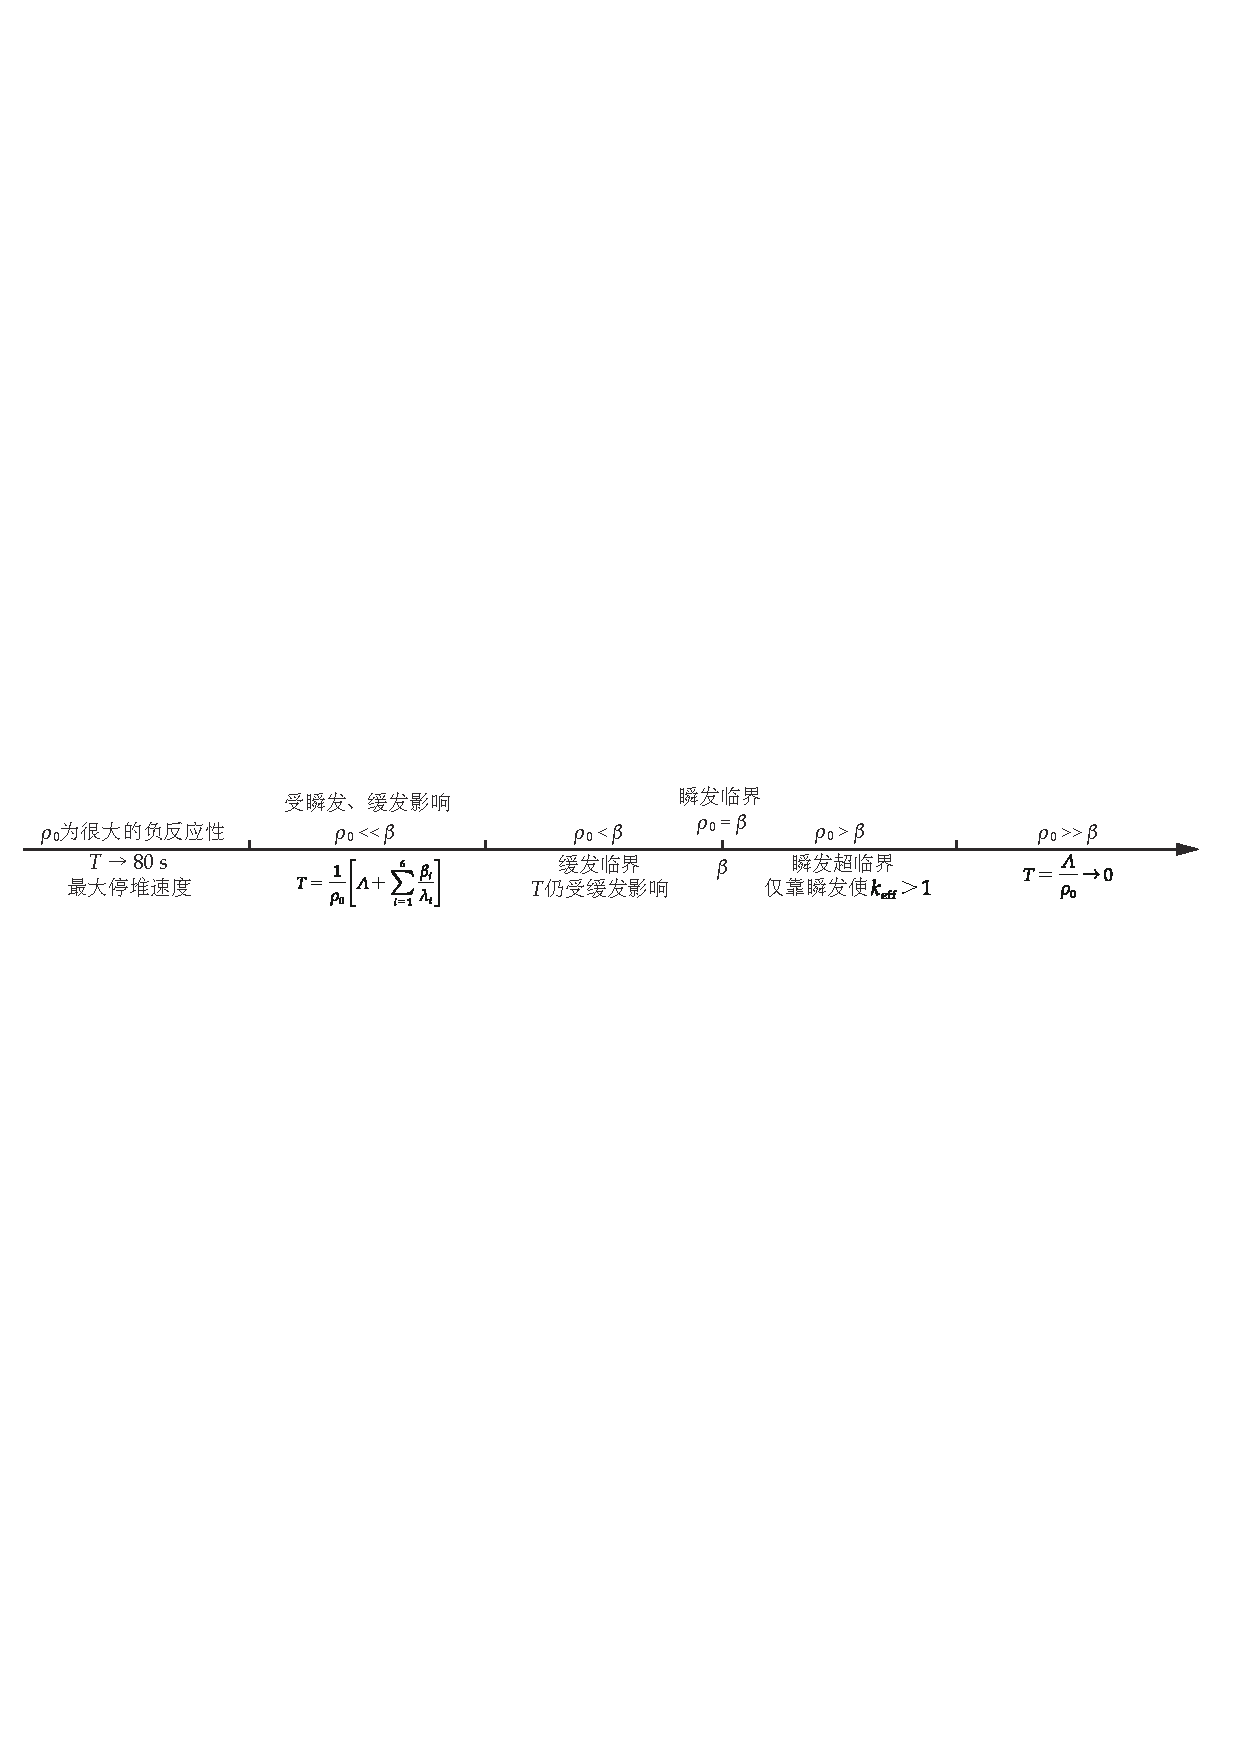
\includegraphics[scale=0.7]{figures/figure4.1.pdf}
\end{figure}

\subsection{核反应堆瞬态响应分析}

本节研究在反应性阶跃输入下,$n(t)$的变化规律。

\subsubsection{六组缓发}

\begin{enumerate}
    \item $\rho > 0$ \quad 开始时$n/n_0$突然上升,然后按缓发中子决定的周期增加;
    \item $\rho < \beta$ \quad 瞬发和缓发中子共同作用才会临界,$n/n0$缓慢上升,时间特性主要由缓发决定;
    \item $\rho < 0$ \quad 开始时$n/n_0$迅速下降,然后按缓发中子决定的速度下降。
\end{enumerate}

\subsubsection{等效单组}

求解过程相当繁琐,建议直接背过方程以应对考试。
\begin{align}
    &n(t) = \frac{n_0}{\beta - \rho_0} \left[\beta {\rm e}^{\frac{\lambda \rho_0}{\beta - \rho_0}t} - \rho_0 {\rm e}^{-\frac{\beta - \rho_0}{\varLambda}t}\right](\text{小阶跃}) \label{little step} \\
    &n(t) = \frac{n_0}{\rho_0 - \beta} \left[\rho_0 {\rm e}^{\frac{\rho_0 - \beta}{\varLambda}t} - \beta {\rm e}^{-\frac{\lambda \rho_0}{\rho_0 - \beta}t}\right](\text{大阶跃}) \label{big step}
\end{align}

常源近似和瞬跳近似了解即可。

\subsection{核反应堆的传递函数}

\begin{definition}[系统的传递函数]
    零初始条件下,线性定常系统输出变量拉普拉斯变换与输入变量拉普拉斯变换之比,表征系统的固有特征。
\end{definition}

\subsubsection{六组缓发}
将\cref{linear equation}做拉普拉斯变换,得
\begin{equation}
    \begin{cases}\displaystyle
        s\Delta N(s) = \frac{n_0}{\varLambda}\Delta \rho(s) + \frac{\rho_0 - \beta}{\varLambda}\Delta N(s) + \sum_{i=1}^{6} \lambda_i \Delta C_i(s) \\
        s\Delta C_i(s) = \frac{\beta_i}{\varLambda} \Delta N(s) - \lambda_i \Delta C_i(s)
    \end{cases}
\end{equation}

解得传递函数为
\begin{equation}
    K_{\rm R} G_{\rm R}(s) = \frac{\Delta N(s)}{\Delta \rho(s)} = \frac{n_0}{\displaystyle s\left(\varLambda + \sum_{i=1}^{6} \frac{\beta_i}{s+\lambda_i}\right) - \rho_0}
\end{equation}

临界时,$\rho_0 = 0$。

\subsubsection{等效单组}
同理对等效单组缓发中子线性化方程进行拉普拉斯变换,解得
\begin{equation}
    K_{\rm R} G_{\rm R}(s) = \frac{\Delta N(s)}{\Delta \rho(s)} = \frac{n_0}{\varLambda s + \frac{\beta s}{s+\lambda} - \rho_0}
\end{equation}

临界时,有
\begin{equation}
    K_{\rm R} G_{\rm R}(s) = \frac{n_0}{\varLambda} \frac{s+\lambda}{s(s+\beta/\varLambda)}
\end{equation}

离散化后,有
\begin{equation}
    K_{\rm R} G_{\rm R}(z) = \frac{n_0 T}{\varLambda} \frac{(z-1)+\lambda T}{(z-1)[(z-1)+\lambda T+\beta T/\varLambda]}
\end{equation}

常源近似和瞬跳近似也是了解即可。

\subsubsection{引入温度反馈}

燃料温度变化引起反应性效应是瞬发的,慢化剂温度变化引起的反应性效应是缓发的。

不必熟练掌握,对照课本推导,知道在题目存在温度反馈时如何使用相关物理量解题即可。

\subsection{核反应堆的频率特性}

\subsubsection{高频段}
$\varomega$增大,幅值减小,相位角$\varphi(\varomega) \to -\pi/2$,当$\varomega$足够大时,$\lambda_i$不再起作用,频率特性与缓发中子无关。

\subsubsection{低频段}
$\varomega$减小,幅值增大,相位角$\varphi(\varomega) \to -\pi/2$。

要能结合结论看懂教材图4-17。

\subsubsection{具有温度反馈}

\begin{enumerate}
    \item 低频段,$K_{\rm RT}G_{\rm RT}(j\varomega) = 1/K_{\rm TC}$,与反应堆无关,只与反馈特性有关;
    \item 高频段,$K_{\rm RT}G_{\rm RT}(j\varomega) = K_{\rm R}G_{\rm R}(j\varomega)$,与反馈特性无关,只与反应堆有关。
\end{enumerate}

\subsection{核反应堆的状态空间表达式}

\subsubsection{等效单组}
由\cref{equal linear}改写,得
\begin{align}
    \begin{bmatrix}
        \Delta \dot{n} \\
        \Delta \dot{c}
    \end{bmatrix} &= \begin{bmatrix}
        -\frac{\beta}{\varLambda} & \lambda \\
        \frac{\beta}{\varLambda} & -\lambda
    \end{bmatrix} \begin{bmatrix}
        \Delta n \\
        \Delta c
    \end{bmatrix} + \begin{bmatrix}
        \frac{n_0}{\varLambda} \\
        0
    \end{bmatrix} \Delta \rho \\
    y &= \begin{bmatrix}
        1 & 0
    \end{bmatrix} \begin{bmatrix}
        \Delta n \\
        \Delta c
    \end{bmatrix}
\end{align}

其与传递函数的关系见\cref{G}。

\subsubsection{反应性阶跃}

由\cref{equal one}改写,得
\begin{equation}
    \begin{bmatrix}
        \dot{n} \\
        \dot{c}
    \end{bmatrix} = \begin{bmatrix}
        \frac{\rho_0 - \beta}{\varLambda} & \lambda \\
        \frac{\beta}{\varLambda} & -\lambda
    \end{bmatrix} \begin{bmatrix}
        n \\
        c
    \end{bmatrix}
\end{equation}

它的近似解正是小阶跃下核反应堆的瞬态响应结果,即\cref{little step}。
\subsection{习题选解}

\begin{exercise} % 4.1
    闭环传递函数标准型为
    \begin{equation*}
        G(s) = \frac{\varomega_n^2}{s^2 + 2\xi \varomega_n s + \varomega_n^2}
    \end{equation*}
    \begin{align*}
        &G_0(s) = \frac{\frac{16}{s+0.8}}{1+\frac{16k}{s+0.8}} = \frac{16}{s+0.8+16k} \\
        &G(s) = \frac{G_0(s)\frac{1}{s}}{1+G_0(s)\frac{1}{s}} = \frac{16}{s^2 + (16k+0.8)s + 16} = \frac{4^2}{s^2 + 2\times 4 \times \frac{16k+0.8}{8}s + 4^2}
    \end{align*}
    由题意,得
    \begin{equation*}
        \xi = \frac{16k+0.8}{8} = 0.5 \Rightarrow k = 0.2
    \end{equation*}
\end{exercise}

\setcounter{exercise}{2}

\begin{exercise} % 4.3
    \begin{equation*}
        G(s) = \frac{U_o(s)}{U_i(s)} = \frac{\frac{1}{sC_2}+R_2}{\frac{1}{sC_1}\Vert R_1 + \frac{1}{sC_2} + R_2} = \frac{(1+sC_1 R_1)(1+sC_2 R_2)}{1+s(C_1 R_1 + C_2 R_2)+s^2 C_1R_1 C_2R_2}
    \end{equation*}
\end{exercise}

\setcounter{exercise}{5}

\begin{exercise} % 4.6
    这里只给出$\rho = 0.001$的情况。
    \begin{enumerate}
        \item 用增量状态空间表达式
        \begin{align*}
            \begin{bmatrix}
                \Delta \dot{n} \\
                \Delta \dot{c}
            \end{bmatrix} &= \begin{bmatrix}
                -\frac{\beta}{\varLambda} & \lambda \\
                \frac{\beta}{\varLambda} & -\lambda
            \end{bmatrix} \begin{bmatrix}
                \Delta n \\
                \Delta c
            \end{bmatrix} + \begin{bmatrix}
                \frac{n_0}{\varLambda} \\
                0
            \end{bmatrix} \Delta \rho \\
            y &= \begin{bmatrix}
                1 & 0
            \end{bmatrix} \begin{bmatrix}
                \Delta n \\
                \Delta c
            \end{bmatrix}
        \end{align*}
        这里输入为$\Delta \rho = 0.001$,代入相关量,得
        \begin{align*}
            \begin{bmatrix}
                \Delta \dot{n} \\
                \Delta \dot{c}
            \end{bmatrix} &= \begin{bmatrix}
                -70 & 0.08 \\
                70 & -0.08
            \end{bmatrix} \begin{bmatrix}
                \Delta n \\
                \Delta c
            \end{bmatrix} + \begin{bmatrix}
                10^4 n_0 \\
                0
            \end{bmatrix} \times 0.001 \\
            (s\symbfit{I} - \symbfit{A})^{-1} &= \frac{\begin{bmatrix}
                s+0.08 & 0.08 \\
                70 & s+70
            \end{bmatrix}}{s(s+70.08)}
        \end{align*}
        \begin{align*}
            {\rm e}^{\symbfit{A}t} &= \mathcal{L}^{-1}\left[(s\symbfit{I} - \symbfit{A})^{-1}\right] = \begin{bmatrix}
                \frac{1}{876}+\frac{875}{876}{\rm e}^{-70.08t} & 0.08+{\rm e}^{-70.08t} \\
                70+{\rm e}^{-70.08t} & \frac{875}{876}+\frac{1}{876}{\rm e}^{-70.08t}
            \end{bmatrix} \\
            \Delta n(t) &= {\rm e}^{\symbfit{A}t} \Delta n(0) + \int_{0}^{t} {\rm e}^{\symbfit{A}(t-\tau)} \begin{bmatrix}
                10n_0 \\
                0
            \end{bmatrix} \times 0.001 {\rm d}\tau \\
            &= 0 + \int_{0}^{t} 10n_0\left[\frac{1}{876}+\frac{875}{876}{\rm e}^{-70.08(t-\tau)}\right] {\rm d}\tau
        \end{align*}
        \item 用动态状态空间表达式
        \begin{equation*}
            \begin{bmatrix}
                \dot{n} \\
                \dot{c}
            \end{bmatrix} = \begin{bmatrix}
                \frac{\rho_0 - \beta}{\varLambda} & \lambda \\
                \frac{\beta}{\varLambda} & -\lambda
            \end{bmatrix} \begin{bmatrix}
                n \\
                c
            \end{bmatrix}
        \end{equation*}
        这里为阶跃$\rho_0 = 0.001$,代入相关量,得
        \begin{equation*}
            \begin{bmatrix}
                \dot{n} \\
                \dot{c}
            \end{bmatrix} = \begin{bmatrix}
                -60 & 0.08 \\
                70 & -0.08
            \end{bmatrix} \begin{bmatrix}
                n \\
                c
            \end{bmatrix}
        \end{equation*}
        参照教材推导流程,解得
        \begin{align*}
            n(t) &= \frac{n_0}{\beta - \rho_0} \left[\beta {\rm e}^{\frac{\lambda \rho_0}{\beta - \rho_0}t} - \rho_0 {\rm e}^{-\frac{\beta - \rho_0}{\varLambda}t}\right] \\
            &= 166.67 n_0 (0.007{\rm e}^{0.01333t}-0.001{\rm e}^{-60t})
        \end{align*}
    \end{enumerate}
    需要说明,这两种方法得到的结果并不相等,因为在推导中取的近似本就不同,相对而言,由动态状态空间表达式得到的解更为准确。
\end{exercise}


\section{核反应堆控制系统的稳定性分析}

请先自行复习《自动控制原理》中闭环特征方程式、根轨迹、奈奎斯特图及判据的相关知识,本章的题目大多是在上学期自控题目的基础上引入了核反应堆控制的背景,会解答具体题目,了解不同类型核反应堆系统的稳定性结论即可应对考试。

\subsection{核反应堆系统稳定性}

根轨迹始终在左半$s$平面,则核反应堆系统稳定。

\subsubsection{两路并联温度反馈}

\begin{enumerate}
    \item $H_{\rm f} + H_{\rm s} > 0$时,系统必不稳定(反馈为正);
    \item $H_{\rm f} + H_{\rm s} < 0$时,系统不一定稳定。
\end{enumerate}

\subsubsection{两路串联温度反馈}

\begin{enumerate}
    \item $\alpha_{\rm f} + \alpha_{\rm m} > 0$,系统必不稳定;
    \item $\alpha_{\rm f} + \alpha_{\rm m} < 0$,系统不一定稳定;
    \item $\alpha_{\rm f}$的效应更快更强。
\end{enumerate}

\subsubsection{石墨气冷动力堆}

反应性慢化剂温度系数上限是
\begin{equation}
    \alpha_{\rm mc} = -\alpha_{\rm f}\frac{K_{\rm fA}}{K_{\rm fB}}
\end{equation}

\begin{enumerate}
    \item 运行初期,$\alpha_{\rm f} < 0$,$\alpha_{\rm m} < 0$,随着燃耗加深,逐渐过渡为$\alpha_{\rm f} < 0$,$\alpha_{\rm m} > 0$;
    \item $\alpha_{\rm m} < \alpha_{\rm mc}$时,系统稳定;$\alpha_{\rm m} > \alpha_{\rm mc}$时,系统不稳定;
    \item 正常运行时,石墨堆天然满足$\alpha_{\rm m} > \alpha_{\rm mc}$,即石墨堆固有不稳定,即使将气体出口温度效应考虑进来也无法改变。
\end{enumerate}

\subsection{实验研究型核反应堆}

需要复习《自动控制原理》中关于降阶简化特征方程的相关知识。

\begin{enumerate}
    \item 重水堆的减速器传递系数$K > 2.064$时,系统不稳定;$K < 2.064$时,系统稳定;
    \item 实验研究堆固有稳定。
\end{enumerate}

\subsection{动力堆稳定性}

动力堆带有位置反馈(控制棒),提高了系统稳定性(稳定域扩大一倍),改善了系统的控制性能(瞬态响应更好)。

动力堆稳定的必要条件是其位置反馈传递系数$K_{\rm f} < K_{\rm fc} = |OA|$,调节动力堆系统稳定性,就是要调节系数$K_C$,使得奈奎斯特图中的$(-1,\,j0)$点落在使系统稳定的范围内。

\subsection{数字控制系统稳定性}

请先自行复习劳斯判据的相关知识,特别是不要忘记其必要条件(闭环特征方程不缺项)。

\begin{figure}[H]
    \centering
    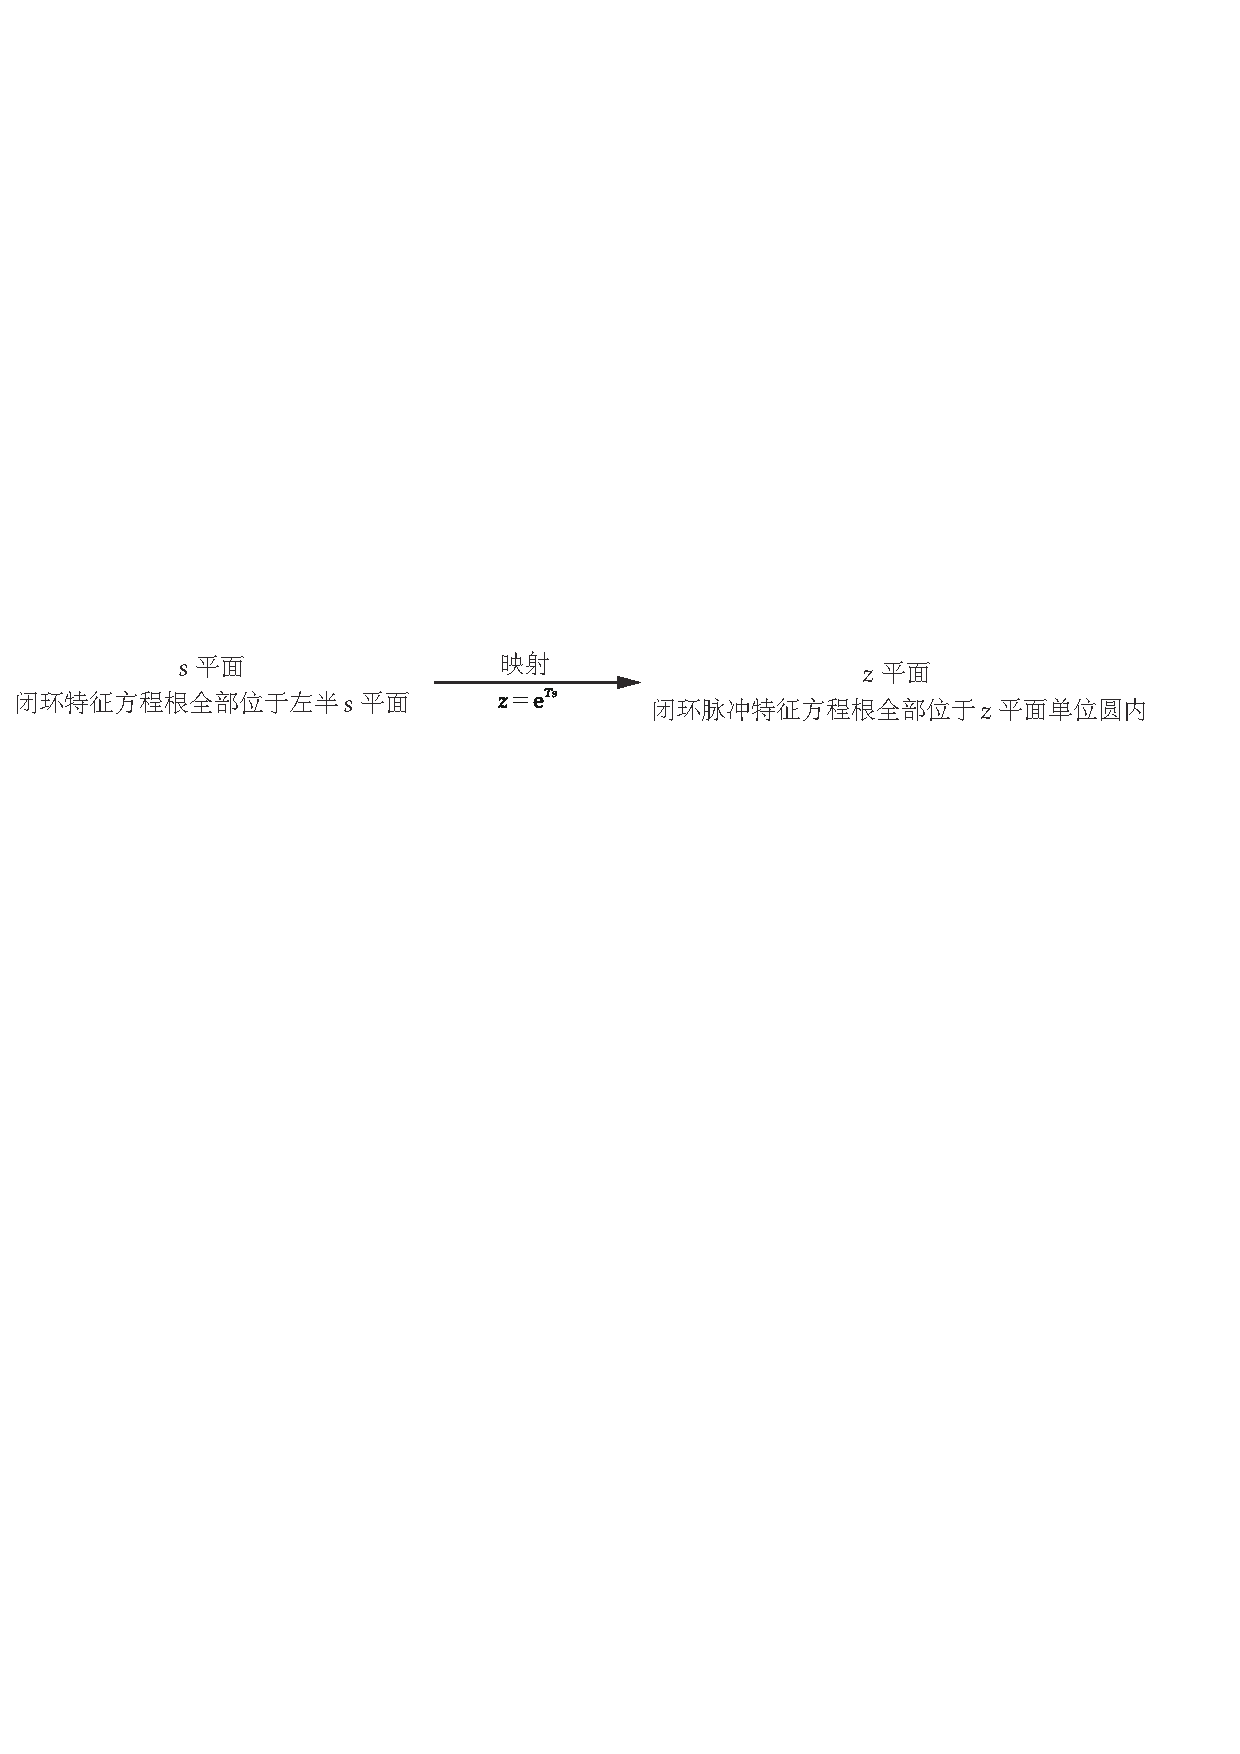
\includegraphics[scale=0.7]{figures/figure5.1.pdf}
\end{figure}

朱利判据了解即可,这里给出两种稳定性判据。

\begin{enumerate}
    \item 直接对闭环脉冲特征方程求解,观察其是否位于$z$平面单位圆内;
    \item 令$w = \frac{z+1}{z-1}$,从$z$平面映射到$w$平面,再使用劳斯判据。
\end{enumerate}

\subsection{核反应堆稳定性状态空间分析}

这里补充实对称矩阵正、负定的判断,具体解题过程参照习题选解。
\begin{enumerate}
    \item 某实对称矩阵$\symbfit{P}$正定 $\Leftrightarrow$ $\symbfit{P}$的所有主子行列式均为正;
    \item 某实对称矩阵$\symbfit{P}$负定 $\Leftrightarrow$ $\symbfit{P}$的奇主子行列式均为负,偶主子行列式均为正。
\end{enumerate}

\subsection{习题选解}

\begin{exercise} % 5.1
    \begin{enumerate}
        \item 令$s=j\varomega$,得
        \begin{align*}
            G(j\varomega)H(j\varomega) &= \frac{K(1-\varomega^2)}{1+\varomega^2} - j\frac{2K\varomega}{1+\varomega^2} \\
            {\rm Re}(\varomega) &= \frac{K(1-\varomega^2)}{1+\varomega^2} \\
            {\rm Im}(\varomega) &= -\frac{2K\varomega}{1+\varomega^2}
        \end{align*}
        \item 起始点,$\varomega \to 0^+$,${\rm Re}(0^+) = K$,${\rm Im}(0^+) = 0^-$;
        终止点,$\varomega \to +\infty$,${\rm Re}(+\infty) = -K$,${\rm Im}(+\infty) = -\infty$
        \item 象限
        \begin{table}[H]
            \centering
            \begin{tabular}{ccc}
                \toprule
                $\varomega$ & $0^+$ & $+\infty$ \\
                \hline
                $K$ & $0^{\circ}$ & $0^{\circ}$ \\
                $1-s$ & $0^{\circ}$ & $-90^{\circ}$ \\
                $\frac{1}{s+1}$ & $0^{\circ}$ & $-90^{\circ}$ \\
                \hline
                $\varphi(\varomega)$ & $0^{\circ}$ & $-180^{\circ}$ \\
                \bottomrule
            \end{tabular}
        \end{table}
        \item 与坐标轴交点
        \begin{enumerate}
            \item ${\rm Im}(\varomega)=0$,$\varomega = 0$(或$\infty$),${\rm Re}(0) = \pm K$,即交点为$(\pm K,\,0)$;
            \item ${\rm Re}(\varomega)=0$,$\varomega = \pm 1$,${\rm Im}(\pm 1) = \mp K$,即交点为$(0,\,\mp K)$。
        \end{enumerate}
        无开环右极点,奈奎斯特图如下。
        \begin{figure}[H]
            \centering
            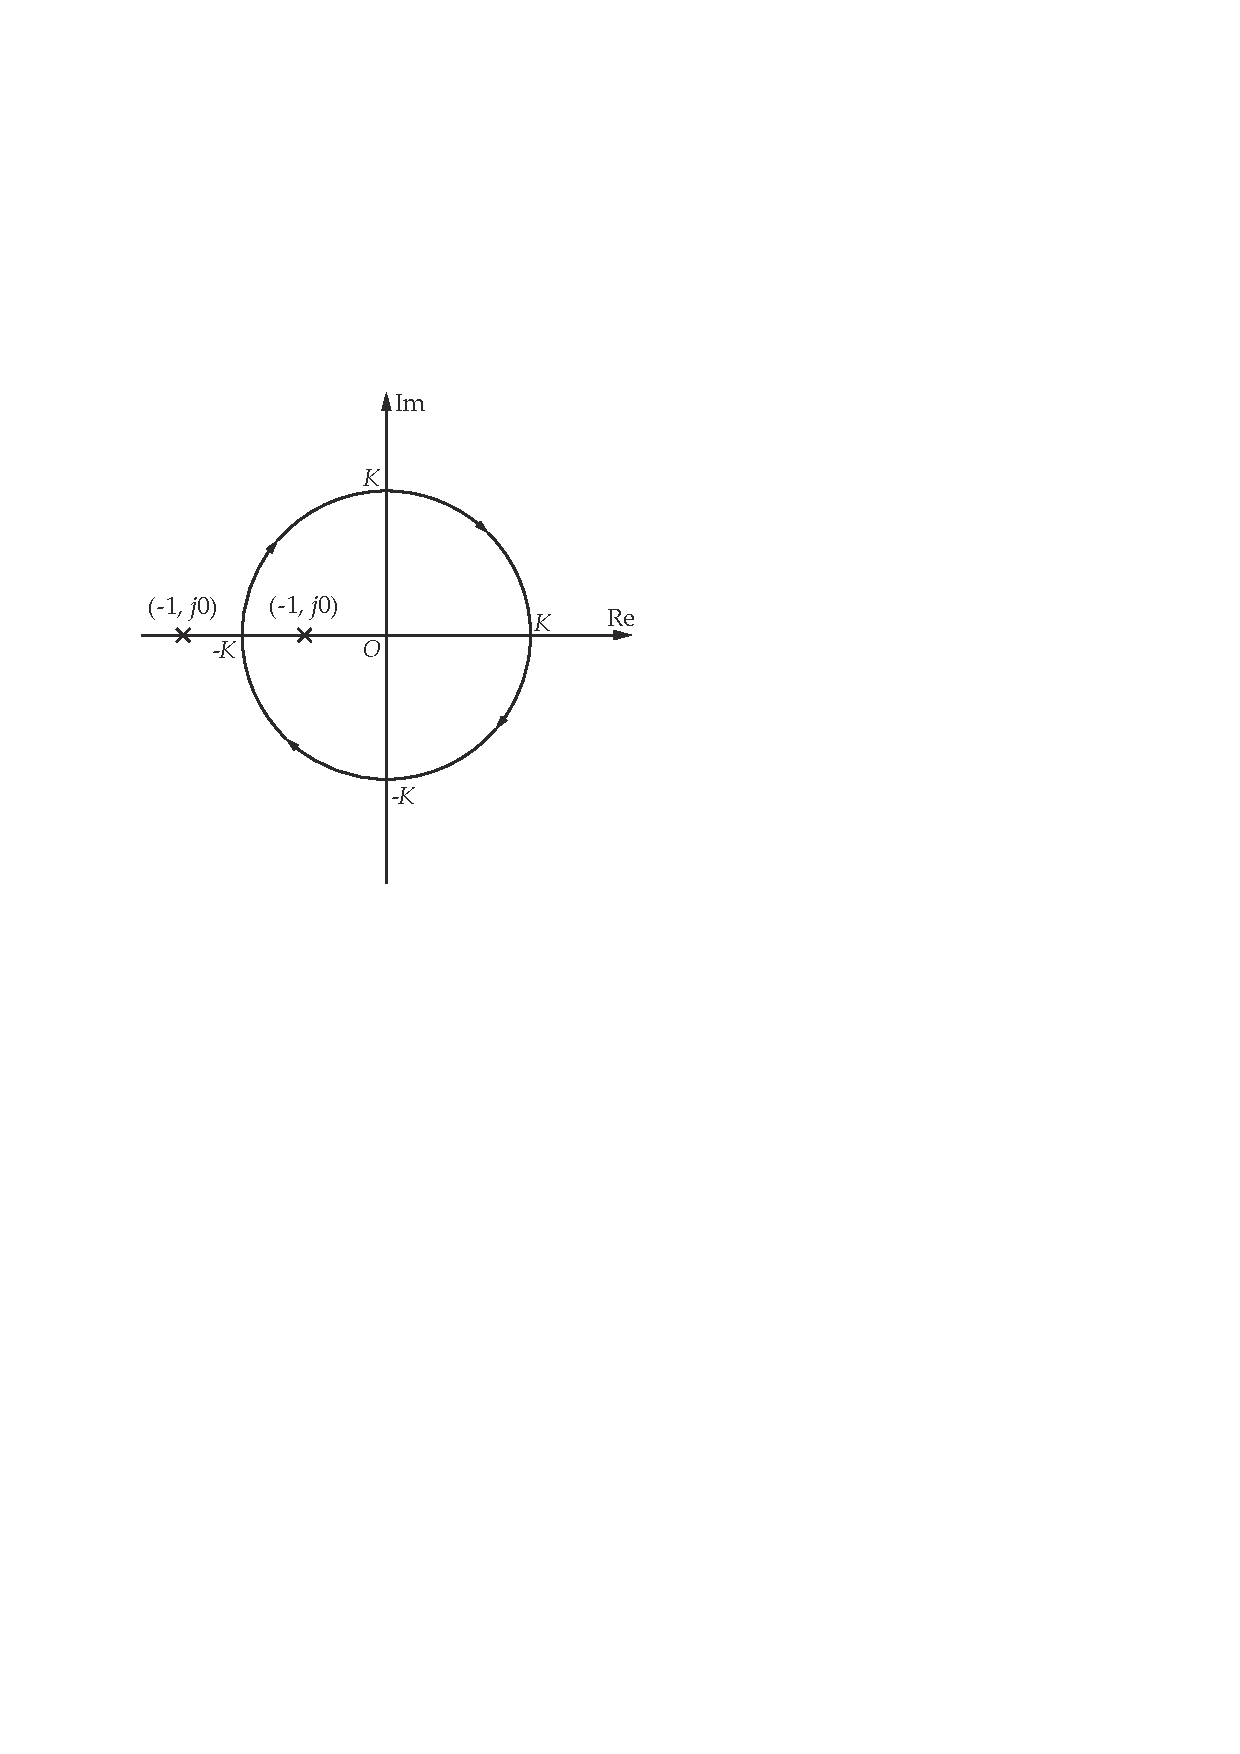
\includegraphics[scale=0.6]{figures/figure5.2.pdf}
        \end{figure}
    \end{enumerate}
    \begin{enumerate}
        \item 若$K<1$,奈奎斯特轨迹不包围$(-1,\,j0)$点,系统闭环稳定;
        \item 若$K\geqslant 1$,奈奎斯特轨迹包围(或经过)$(-1,\,j0)$点,系统闭环不稳定。
    \end{enumerate}
\end{exercise}

\begin{exercise} % 5.2
    \begin{enumerate}
        \item $z_1 = 0.5+0.6181i$,$z_2 = 0.5-0.6181i$,均在$z$平面单位圆内,系统稳定;
        \item $z_1 = -0.5123$,$z_2 = 1.487$,$z_3 = 0.5250$,$z_2$不在$z$平面单位圆内,系统不稳定;
        \item $z_1 = 0.5$,$z_2 = 0.5+0.5i$,$z_3 = 0.5-0.5i$,均在$z$平面单位圆内,系统稳定。
    \end{enumerate}
    或使用劳斯判据。
\end{exercise}

\begin{exercise} % 5.3
    \begin{align*}
        G(z) &= \Z{\frac{1-{\rm e}^{Ts}}{s} \cdot \frac{1}{s(s+1)}} = (1-z^{-1})\left[\frac{1}{s^2(s+1)}\right] \\
        &= (1-z^{-1})\Z{\frac{1}{s^2} - \frac{1}{s} + \frac{1}{s+1}} = (1-z^{-1})\left[\frac{zT}{(z-1)^2} - \frac{z}{z-1} + \frac{z}{z-{\rm e}^{-T}}\right] \\
        &= \frac{zT(z-{\rm e}^{-T})-z(z-1)(z-{\rm e}^{-T})+z(z-1)^2}{z(z-1)(z-{\rm e}^{-T})}
    \end{align*}
    由题意,$T=1\,{\rm s}$,则
    \begin{equation*}
        G(z) = \frac{0.3679z + 0.2642}{z^2-1.3679z+0.3679}
    \end{equation*}
    闭环特征方程$D(z) = z^2 - z + 0.6321$,解得$z=0.5 \pm 0.6181j$,均在$z$平面单位圆内,系统稳定。
\end{exercise}

\setcounter{exercise}{7}

\begin{exercise} % 5.8
    \begin{enumerate}
        \item $\gamma = 0.01\,{\rm s}^{-1}$时,$K_{\rm R}G_{\rm R}(s)H(s) = \frac{K(s+0.1)}{s(s+0.01)(s+100)}$
        \begin{enumerate}
            \item 起始点:$z_1 = 0$,$z_2 = -0.01$,$z_3 = -100$;
            终止点:$p_1 = -0.1$;
            \item 实轴上的根轨迹:$[-100,\,-0.1]$,$[-0.01,\,0]$;
            \item 分支数为3,两支终止于无穷远处;
            \item 渐近线
            \begin{align*}
                -\sigma_a &= -\frac{-0.1-(0-0.01-100)}{3-1} = -49.955 \\
                \theta_k &= \frac{\pm (2k+1)\pi}{3-1} = \begin{cases}
                    \pm \frac{\pi}{2},\,k=0 \\
                    \pm \frac{3\pi}{2},\,k=1
                \end{cases}
            \end{align*}
            \item 分离点与会合点
            闭环特征方程$s(s+0.01)(s+100)+K(s+0.1) = 0$,于是有
            \begin{equation*}
                K = -\frac{s(s+0.01)(s+100)}{s+0.1}
            \end{equation*}
            令$\dv{K}{s} = 0$,得
            \begin{equation*}
                2s^3 + 100.31s^2 + 20.002s + 0.1 = 0 \Rightarrow \begin{cases}
                    s_1 = -49.955 \\
                    s_2 = -0.00513 \\
                    s_3 = -0.195
                \end{cases}
            \end{equation*}
            其中,$s_1$和$s_2$为分离点,$s_3$为会合点。
            \item 与虚轴的交点
            闭环特征方程中令$s=-j\varomega$,得
            \begin{equation*}
                -j\varomega^3 - 100.01\varomega^2 + (1+K)j\varomega + 0.1K = 0 \Rightarrow \begin{cases}
                    \varomega^3 - (1+K) \varomega = 0 \\
                    100.01\varomega^2 - 0.1K = 0
                \end{cases} \Rightarrow \begin{cases}
                    K = 0 \\
                    \varomega = 0
                \end{cases}
            \end{equation*}
            只与原点相交。
        \end{enumerate}
        故,根轨迹如下。
        \begin{figure}[H]
            \centering
            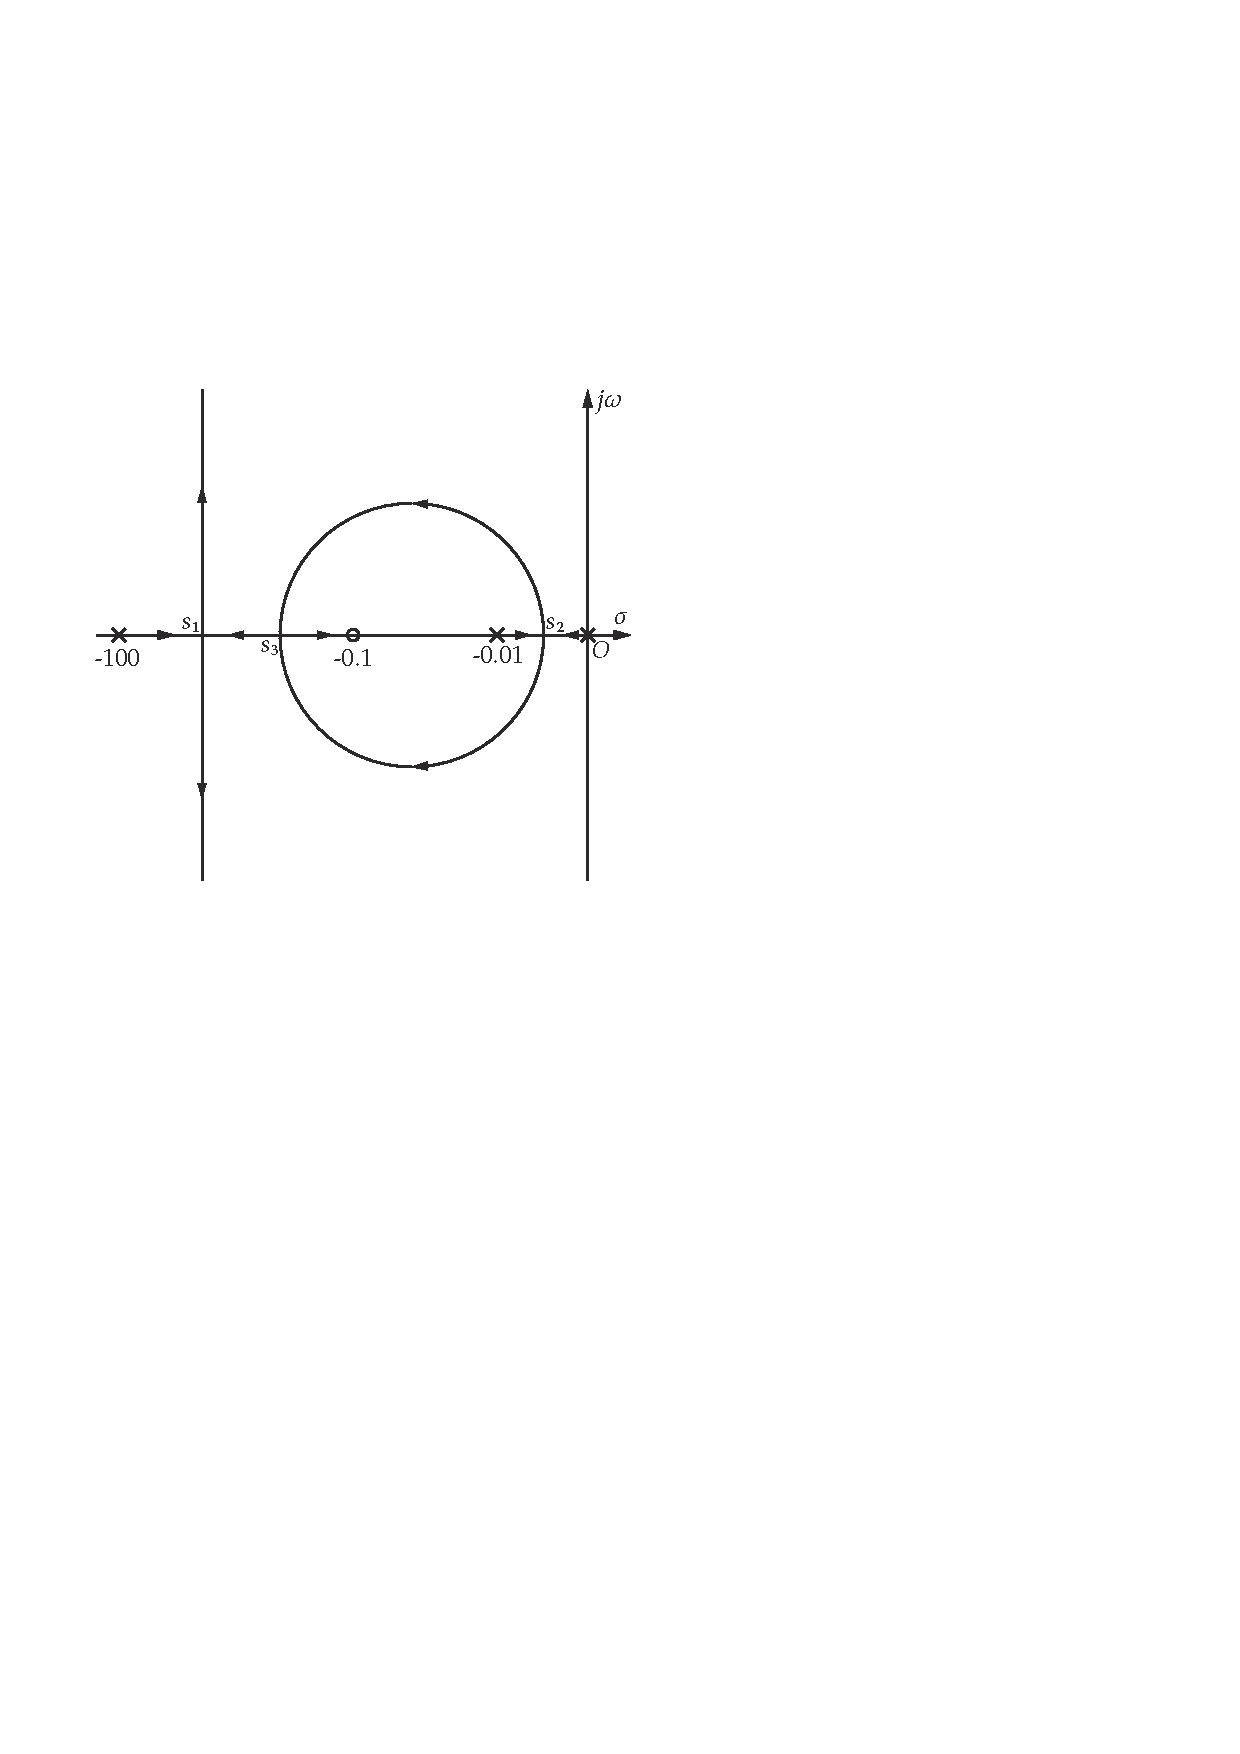
\includegraphics[scale=0.6]{figures/figure5.3.pdf}
        \end{figure}
        \item $\gamma = 1\,{\rm s}^{-1}$时,$K_{\rm R}G_{\rm R}(s)H(s) = \frac{K(s+0.1)}{s(s+1)(s+100)}$
        \begin{enumerate}
            \item 起始点:$z_1 = 0$,$z_2 = -1$,$z_3 = -100$;
            终止点:$p_1 = -0.1$;
            \item 实轴上的根轨迹:$[-100,\,-1]$,$[-0.1,\,0]$;
            \item 分支数为3,两支终止于无穷远处;
            \item 渐近线
            \begin{align*}
                -\sigma_a &= -\frac{-0.1-(0-1-100)}{3-1} = -50.45 \\
                \theta_k &= \frac{\pm (2k+1)\pi}{3-1} = \begin{cases}
                    \pm \frac{\pi}{2},\,k=0 \\
                    \pm \frac{3\pi}{2},\,k=1
                \end{cases}
            \end{align*}
            \item 分离点与会合点
            闭环特征方程$s(s+1)(s+100)+K(s+0.1) = 0$,于是有
            \begin{equation*}
                K = -\frac{s(s+1)(s+100)}{s+0.1}
            \end{equation*}
            令$\dv{K}{s} = 0$,得
            \begin{equation*}
                2s^3 + 101.3s^2 + 20.2s + 10 = 0 \Rightarrow \begin{cases}
                    s_1 = -50.45 \\
                    s_{2,3} = -0.1 \pm 0.3j
                \end{cases}
            \end{equation*}
            其中,$s_1$为分离点。
            \item 与虚轴的交点
            闭环特征方程中令$s=-j\varomega$,得
            \begin{equation*}
                -j\varomega^3 - 101\varomega^2 + (100+K)j\varomega + 0.1K = 0 \Rightarrow \begin{cases}
                    \varomega^3 - (100+K) \varomega = 0 \\
                    101\varomega^2 - 0.1K = 0
                \end{cases} \Rightarrow \begin{cases}
                    K = 0 \\
                    \varomega = 0
                \end{cases}
            \end{equation*}
            只与原点相交。
        \end{enumerate}
        故,根轨迹如下。
        \begin{figure}[H]
            \centering
            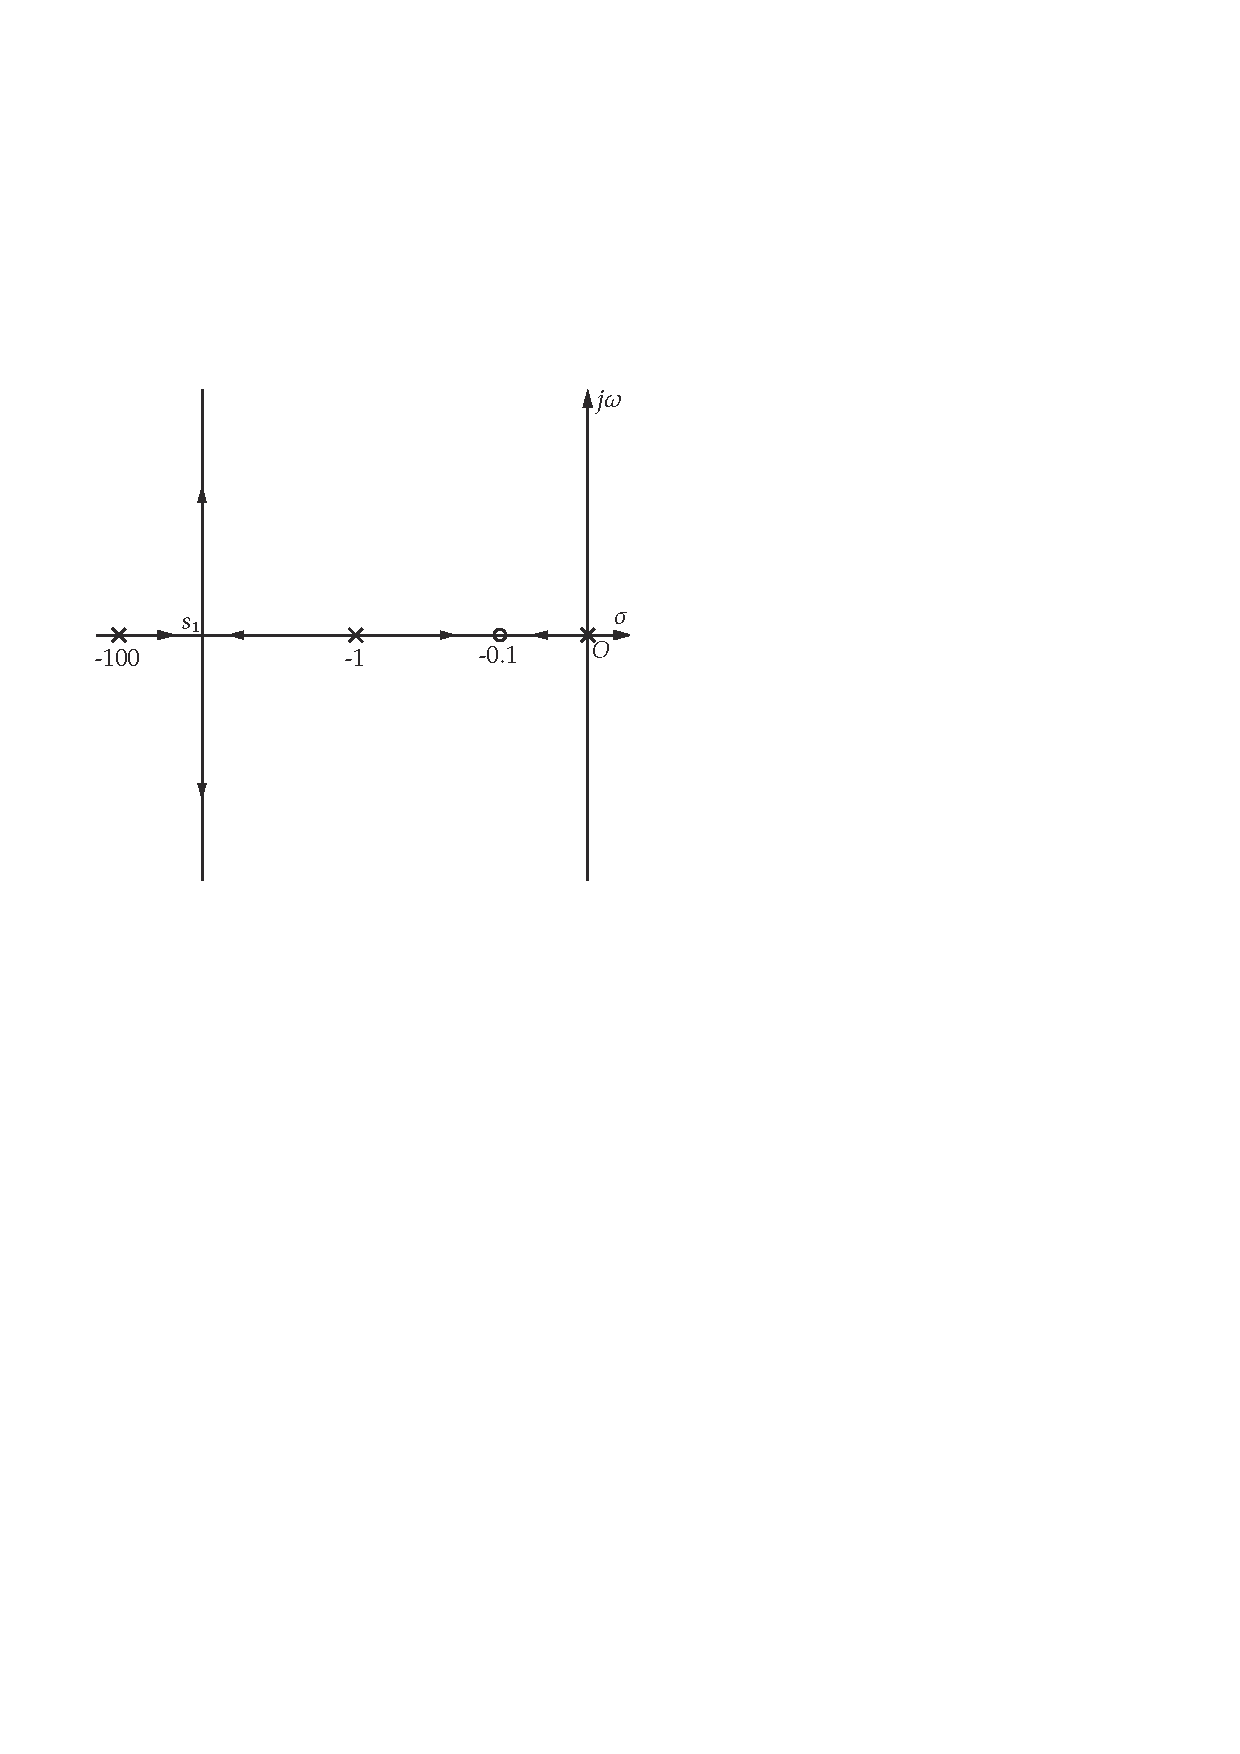
\includegraphics[scale=0.6]{figures/figure5.4.pdf}
        \end{figure}
    \end{enumerate}
\end{exercise}

\setcounter{exercise}{10}

\begin{exercise} % 5.11
    \begin{enumerate}
        \item 未考虑功率负反馈时
        \begin{equation*}
            \begin{cases}
                \dv{\Delta n}{t} = \frac{n_0}{\varLambda}\Delta \rho + \frac{\rho_0 - \beta}{\varLambda}\Delta n + \lambda \Delta c \\
                \dv{\Delta c}{t} = \frac{\beta}{\varLambda}\Delta n - \lambda \Delta c
            \end{cases}
        \end{equation*}
        \begin{equation*}
            \begin{bmatrix}
                \Delta \dot{n} \\
                \Delta \dot{c}
            \end{bmatrix} = \begin{bmatrix}
                -\frac{\beta}{\varLambda} & \lambda \\
                \frac{\beta}{\varLambda} & -\lambda
            \end{bmatrix} \begin{bmatrix}
                \Delta n \\
                \Delta c
            \end{bmatrix} + \begin{bmatrix}
                \frac{n_0}{\varLambda} \\
                0
            \end{bmatrix} \Delta \rho 
        \end{equation*}
        代入参量,得
        \begin{equation*}
            \symbfit{A} = \begin{bmatrix}
                -1.067 & 0.1 \\
                1.067 & -0.1
            \end{bmatrix}
        \end{equation*}
        李雅普诺夫函数$V(x) = x^{\top} \symbfit{P} x$,令$\symbfit{Q} = \symbfit{I}$,则$\symbfit{A}^{\top}\symbfit{P} + \symbfit{P}\symbfit{A} = -\symbfit{I}$,即
        \begin{equation*}
            \begin{bmatrix}
                -1.067 & 1.067 \\
                0.1 & -0.1
            \end{bmatrix} \begin{bmatrix}
                p_{11} & p_{12} \\
                p_{21} & p_{22}
            \end{bmatrix} + \begin{bmatrix}
                p_{11} & p_{12} \\
                p_{21} & p_{22}
            \end{bmatrix} \begin{bmatrix}
                -1.067 & 0.1 \\
                1.067 & -0.1
            \end{bmatrix} = \begin{bmatrix}
                -1 & 0 \\
                0 & 1
            \end{bmatrix}
        \end{equation*}
        解得
        \begin{equation*}
            \symbfit{P} = \begin{bmatrix}
                -2.009 & -2.478 \\
                -2.478 & -2.522
            \end{bmatrix}
        \end{equation*}
        该矩阵负定\footnote{该矩阵为手算的近似解,计算器可能显示无解,无论写哪个,只要说明了系统非大范围渐进稳定即可。},即系统在原点处平衡状态非大范围渐进稳定。
        \item 考虑功率负反馈时
        \begin{equation*}
            \begin{cases}
                \dv{\Delta n}{t} = \frac{n_0}{\varLambda}\Delta \rho + \frac{\rho_0 - \beta}{\varLambda}\Delta n + \lambda \Delta c \\
                \dv{\Delta c}{t} = \frac{\beta}{\varLambda}\Delta n - \lambda \Delta c \\
                \Delta \rho = \Delta \rho_{\rm ex} - \alpha_{\rm P} \Delta n
            \end{cases}
        \end{equation*}
        \begin{equation*}
            \begin{bmatrix}
                \Delta \dot{n} \\
                \Delta \dot{c}
            \end{bmatrix} = \begin{bmatrix}
                -\frac{\beta+n_0 \alpha_{\rm P}}{\varLambda} & \lambda \\
                \frac{\beta}{\varLambda} & -\lambda
            \end{bmatrix} \begin{bmatrix}
                \Delta n \\
                \Delta c
            \end{bmatrix} + \begin{bmatrix}
                \frac{n_0}{\varLambda} \\
                0
            \end{bmatrix} \Delta \rho_{\rm ex} 
        \end{equation*}
        同理,解得
        \begin{equation*}
            \symbfit{P} = \begin{bmatrix}
                303.8 & 307.9 \\
                307.9 & 312.9
            \end{bmatrix}
        \end{equation*}
        该矩阵正定,即系统在原点处平衡状态非大范围渐进稳定。
    \end{enumerate}
\end{exercise}

\section{压水堆核电厂控制}

因本章涉及知识比较杂,这里先给出习题选解,再补充一些问答题,关于备考的建议是把作业题搞懂,再仔细看一遍本章的课本内容。

\subsection{习题选解}

\setcounter{exercise}{1}

\begin{exercise} % 6.2
    \begin{enumerate}
        \item 自稳特性是指核反应堆内、外有反应性扰动时,核反应堆能依靠自身内部温度反馈而维持稳定状态的特性;
        \item 自调特性是指核电厂负荷变化时,核反应堆靠自身内部温度反馈使其功率达到与负荷一致的水平,产生新的热平衡。
    \end{enumerate}
\end{exercise}

\setcounter{exercise}{3}

\begin{exercise} % 6.4
    \begin{enumerate}
        \item 经济性:燃料平均燃耗越深,燃料利用越充分;
        \item 安全性:为防止燃料包壳烧毁或堆芯熔化,堆芯最大线功率密度受限;
        \item 正常运行中,线功率密度过高,一旦发生LOCA,也可能超过燃料元件安全容许极限。
    \end{enumerate}
\end{exercise}

\begin{exercise} % 6.5
    \begin{enumerate}
        \item 偏离泡核沸腾准则:核反应堆在正常运行工况下,不应达到DNB点;
        \item 燃料不熔化准则:堆芯线功率密度应小于$590\,{\rm W \cdot cm^{-1}}$;
        \item 失水事故准则:在发生LOCA的情况下,应避免燃料包壳熔化。
    \end{enumerate}
\end{exercise}

\begin{exercise} % 6.6
    \begin{enumerate}
        \item 功率控制系统输入模拟信号(最终功率设定值、操纵员蒸汽流量限值等)和逻辑信号(蒸汽排放系统设置压力控制模式、汽轮机脱扣信号等);
        \item 功率控制系统输出信号有控制棒插入、提升和移动速度信号等;
        \item 输入和输出之间没有反馈环节关联,因此功率补偿棒控制系统是开环控制系统。
    \end{enumerate}
\end{exercise}

\begin{exercise} % 6.7
    当出现一个动态功率失配信号而冷却剂平均温度尚无明显变化时,产生一个超前的控制信号对R棒组进行控制,加速核反应堆对汽轮机负荷需求的响应。
\end{exercise}

\begin{exercise} % 6.8
    以升功率的阶跃变化为例。
    \begin{enumerate}
        \item 负荷阶跃上升,核反应堆要跟踪负荷变化;
        \item 补偿棒定值单元给出对应棒位,功率补偿棒${\rm G_1}$棒组依此提升至响应位置;
        \item 负荷阶跃产生功率失配信号,同时冷却剂平均温度参考值变化使温度偏差$T_e$上升,R棒提升;
        \item 堆内正反应性快速增加,$T_e$落入棒速程序控制单元死区内时R棒停止,但${\rm G_1}$仍在提升;
        \item $T_e$减小到超出死区,R棒开始下插抵消${\rm G_1}$提升的效应;
        \item 直到R棒处于稳定位置,堆内反应性达到平衡。
    \end{enumerate}
\end{exercise}

\begin{exercise} % 6.9
    \begin{enumerate}
        \item 原理:通过供给一回路必要数量的接近于当时慢化剂硼浓度的含硼溶液并将此补充液注入上充泵汲入口处,调节慢化剂硼浓度(稀释/硼化)以控制堆芯反应性。
        \item 作用:
        \begin{enumerate}
            \item 减少了控制棒数量;
            \item 改善了轴向功率分布;
            \item 可增大核反应堆后备反应性,使核反应堆寿期延长,燃耗增加;
            \item 简化堆芯结构。
        \end{enumerate}
    \end{enumerate}
\end{exercise}

\begin{exercise} % 6.10
    \begin{enumerate}
        \item 原理:通过调节并联安装在每条给水管路上的两个调节阀阀门开度控制给水流量,从而实现液位控制;
        \item 特点:
        \begin{enumerate}
            \item 存在蒸汽流量与给水流量的失配信号;
            \item 由主通道、旁路通道和前馈通道组成;
            \item 蒸汽流量、给水流量和液位偏差三参量控制。
        \end{enumerate}
    \end{enumerate}
\end{exercise}

\begin{exercise} % 6.11
    \begin{enumerate}
        \item 原理:上充流量与下泄流量差值为正时液位上升,为负时液位下降,差值绝对值的大小会影响液位变化的快慢;
        \item 特点:液位控制器与上充流量控制器串联。
    \end{enumerate}
\end{exercise}

\begin{exercise} % 6.12
    \begin{enumerate}
        \item 温度控制模式;
        \item 压力控制模式。
    \end{enumerate}
\end{exercise}

\subsection{补充题目}

\begin{enumerate}
    \item 压水堆核电厂控制系统主要功能(P139);
    \item 控制棒和慢化剂中可溶性毒物的作用(P141);
    \item 圆柱形均匀裸堆的功率分布形状(P143);
    \item 【2023填空第一道】R棒、N棒、G棒、黑体棒和灰体棒(P155);
    \item 稳压器的稳压原理(P180)。
\end{enumerate}

\end{document}
\endinput
%%
%% xelatex --synctex=1 main.tex
